\section{Applications}

\subsection{Automating the Scientific Workflow} \label{sec:ai-scientists}

Recent advances in \glspl{gpm}, particularly \glspl{llm}, have enabled initial demonstrations of fully autonomous \gls{ai} scientists \autocite{schmidgall2025agent}. 
We define these as \gls{llm}-powered architectures capable of executing end-to-end research workflows based solely on the final objectives, e.g., \enquote{\textit{Unexplained rise of antimicrobial resistance in Pseudomonas. Formulate hypotheses, design confirmatory in vitro assays, and suggest repurposing candidates for liver-fibrosis drugs}}. 
Such systems navigate partially or entirely through all components of the scientific process outlined in \Cref{fig:applications}, and detailed in the subsequent sections. 

While significant applications emerge in \gls{ml} and programming, scientific implementations remain less explored.

\subsubsection{Coding and ML Applications of AI Scientists}

Notable frameworks, including \modelname{Co-Scientist} \autocite{gottweis2025towards}, and \modelname{\gls{ai}-Scientist} \autocite{yamada2025ai}, aim to automate the entire \gls{ml} research pipeline, typically employing multi-agent architectures (described in detail in \Cref{sec:multi-agent}) where specialized agents manage distinct phases of the scientific method \autocite{schmidgall2025agentrxiv}. 
Critical to these systems is self-reflection \autocite{renze2024self0reflection}---iterative evaluation and criticism of results within validation loops. 
However, comparative analyses reveal that \gls{llm}-based evaluations frequently overscore outputs relative to human assessments \autocite{huang2023mlagentbench0, chan2024mle, starace2025paperbench0}. 
From an engineering perspective, alternative approaches focus specifically on iterative code optimization, enabling systems to refine their codebases \autocite{zhang2025darwin} or generate improved agents autonomously \autocite{hu2024automated}.
In another work, \modelname{AlphaEvolve} \autocite{novikov2025alphaevolve}, which is an \gls{llm} operating within a \gls{ga} environment, found novel algorithms for matrix multiplication (which had seen no innovation in fifty years) and sorting.

\subsubsection{Chemistry and Related Fields}

In chemistry, proposed systems show promising results. \modelname{Robin} identified ripasudil as a treatment for \gls{damd} \autocite{ghareeb2025robin0}---despite pending clinical trials and the general debate for these systems about novelty of their findings\autocite{Listgarten2024perpetual}.
However, automation of experiment execution poses a major constraint for the chemistry-focused \gls{ai}-scientists due to hardware requirements, making computational chemistry the most feasible subfield in which agents have successfully run simple quantum simulations \autocite{Zou2025ElAgente}. 
Further, the \glspl{llm} powering these systems exhibit limited chemical knowledge \autocite{mirza2024large}. 
Despite this, \modelname{ether0} \autocite{narayanan2025training}---the first chemistry-specialized reasoning \gls{llm} (see \Cref{sec:rl} for a deeper discussion on reasoning models)---demonstrated strong capabilities in molecular design and accurate reaction prediction, positioning it as a promising foundation for chemistry-focused \gls{ai} scientists.

\subsubsection{Are these Systems Capable of Real Autonomous Research?}

Although agents like \modelname{Zochi} \autocite{intologyai2025zochi} achieved peer-reviewed publication in top-tier venues (\gls{acl} 2025), their capacity for truly autonomous end-to-end research remains debatable \autocite{son2025ai}. 
Even when generating hypotheses that appear novel and impactful, their execution and reporting of these ideas, as demonstrated by \textcite{si2025ideation1execution}, yield results deemed less attractive than those produced by humans. Additionally, this autonomy raises a critical question: \textit{What should the role of \gls{ai} in science be?} 
While these systems can generate hypotheses, conduct experiments, and produce publication-ready manuscripts, their integration demands careful consideration (refer to \Cref{sec:ethics} for further discussion about moral concerns around these systems). 
Beyond the vision of fully autonomous scientists, \glspl{gpm}---primarily \glspl{llm}---are already utilized across most scientific workflow components, for which \glspl{llm} have proven useful for some. 
These elements are shown in \Cref{fig:applications}, and we discuss next.


\begin{figure}[!ht]
    \centering
    \label{fig:applications}
    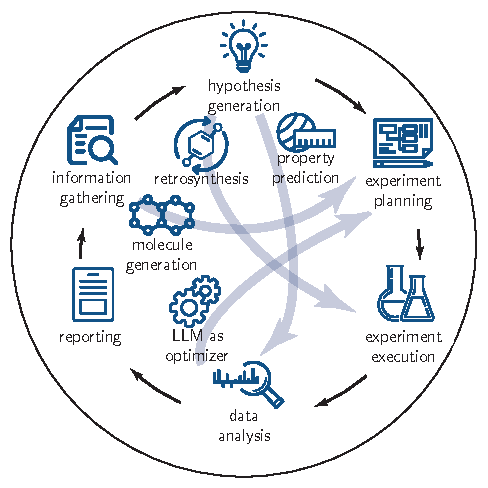
\includegraphics[width=0.5\textwidth]{figures/rescaled_figures/chemrev_figure11.pdf}
    \caption{\textbf{Overview of the scientific process}. The outer elements represent the typical scientific research process: from gathering information and generating hypotheses based on the observations, to executing experiments and analyzing the results. The terms that are in the center represent data-driven \enquote{shortcuts} that \enquote{accelerate} the typical scientific method. All stages represented in the figure are discussed in detail in the following sections.}
\end{figure}

\subsection{Existing GPMs for Chemical Science}

The development of \glspl{gpm} for chemical science represents a departure from traditional single-task approaches. Rather than fine-tuning pre-trained models for specific applications such as property prediction or molecular generation, these chemistry-aware language models are intentionally designed to perform multiple chemical tasks simultaneously. This multitask paradigm offers several advantages: shared representations across related chemical problems\autocite{dimitrios2023unifying}, improved data efficiency through transfer learning between tasks\autocite{lim2021predicting}, and the potential for emergent capabilities that arise from joint training across diverse chemical domains\autocite{livne2024nach0}.

\paragraph{Multitask Learning Frameworks} \modelname{DARWIN 1.5} pioneered the multitask approach by fine-tuning \modelname{Llama-7B} through a two-stage process \autocite{xie2025darwin}. Initially trained on 332k scientific question-answer pairs to establish foundational scientific reasoning, the model subsequently underwent multitask learning to perform property prediction-related regression and classification tasks concurrently.

Building on similar principles, \modelname{nach0} introduced a unified encoder-decoder transformer architecture for cross-domain chemical tasks \autocite{livne2024nach0}. Pre-trained using \gls{ssl} on both natural language and chemical data, \modelname{nach0} tackles diverse downstream applications including molecular structure generation, chemical property prediction, and reaction prediction. Notably, the authors found that combining chemistry-specific tasks outperformed models trained on distinct task groups, suggesting that chemical reasoning benefits from focused domain integration.

In the materials domain, \textcite{qu2023leveraging} developed a language-driven materials discovery framework that uses transformer-based embeddings (e.g., \modelname{MatBERT}\autocite{wan2024tokens}) to represent and generate novel crystal structures. Candidates are first recalled via similarity in embedding space, then ranked using a multitask multi-gate \gls{moe} model that predicts the desired properties jointly. 
Their method successfully identifies novel high-performance materials (e.g., halide perovskites) and demonstrates that language representations encode latent knowledge for task-agnostic materials design.

\paragraph{Domain-Specific Pre-Training Strategies} A second category of \glspl{gpm} emphasizes deep domain knowledge through specialized pre-training. \modelname{LLaMat} employed \gls{peft} specifically on crystal structure data in \gls{cif} format, enabling the generation of thermodynamically stable structures \autocite{mishra2024foundational}.

\modelname{ChemDFM} scales this concept significantly, implementing domain pre-training on over 34 billion tokens from chemical textbooks and research articles \autocite{zhao2024chemdfm}. Through comprehensive instruction tuning, \modelname{ChemDFM} familiarizes itself with chemical notation and patterns, distinguishing it from more materials-focused approaches like \modelname{LLaMat} through its broader chemical knowledge base.

\modelname{ChemLLM} further refined this approach by introducing template-based instruction tuning (ChemData) to optimize property-guided molecular generation \autocite{zhang2024chemllm}.

\paragraph{Reasoning-Based Approaches} A recent development in chemical \glspl{gpm} incorporates explicit reasoning capabilities. \modelname{ether0} demonstrates this approach as a 24 billion parameter reasoning model trained on over 640k experimentally-grounded chemistry problems across diverse tasks, including retrosynthesis, solubility editing, and property prediction \autocite{narayanan2025training}. 
Unlike previous models, \modelname{ether0} uses \gls{rl} (see \Cref{sec:rl}) to develop reasoning behaviors like verification and backtracking, demonstrating that structured problem-solving approaches can significantly improve performance on complex chemical tasks while maintaining grounding in experimental data.

These diverse approaches illustrate the evolving landscape of chemical \glspl{gpm}, each balancing broad applicability with domain-specific precision.
Still, most applications of \glspl{gpm} focus on using these models for one specific application and we will review those in the following.

\subsection{Knowledge Gathering}\label{sec:information_gathering}
The rate of publishing keeps growing, and as a result, it is increasingly challenging to manually collect all relevant knowledge, potentially stymying scientific progress.\autocite{schilling2025text, Chu_2021}
Even though knowledge collection might seem like a simple task, it often involves multiple different steps, visually described in \Cref{fig:knowledge_gathering}. We split the discussion in this section in two: structured data extraction and question answering. Example queries for both sections are in \Cref{fig:knowledge_gathering}B.

\begin{figure}[!ht]
    \centering
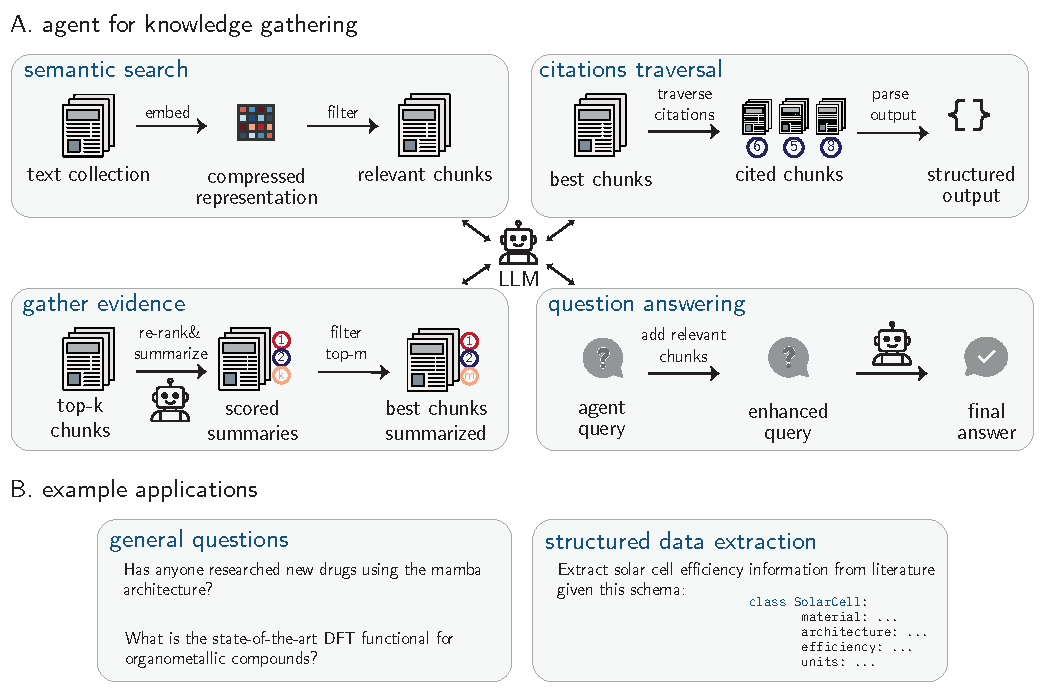
\includegraphics[width=1\textwidth]{figures/rescaled_figures/chemrev_figure12.pdf}
    \caption{\textbf{A. a representation of a typical agent for scientific queries.} The \gls{llm} is the central piece of the system, surrounded by typical tools that improve its question-answering capabilities, together forming an agentic system. The tools represented in this figure are semantic search, citation traversal, evidence gathering, and question answering. Semantic search finds relevant documents. Evidence gathering ranks and filters chunks of text using \glspl{llm}. The citation traversal tool provides model access to citation graphs, enabling accurate referencing of each chunk and facilitating the discovery of additional sources. Finally, the question-answering tool (an \gls{llm}) collects all the information found by other tools and generates a final response to a user's query. This part the figure is inspired by the \modelname{PaperQA2} agent.\autocite{skarlinski2024language} \textbf{B.} two examples of applications discussed in this section.}
\label{fig:knowledge_gathering}
\end{figure}


\paragraph{Semantic Search} A step that is key to most, if not all, knowledge-gathering tasks is \gls{rag}, discussed in more detail in \Cref{sec:rag}. 
Most commonly, this involves semantic search, intended to identify chunks of text with similar meaning. 
The difference between semantic search and conventional search lies in how each approach interprets queries. The latter operates through lexical matching---whether exact or fuzzy---focusing on the literal words and their variations. Semantic search, however, goes deeper by interpreting the underlying meaning and contextual relationships within the content. 

To enable semantic search, documents are stored in vector databases using embedding vectors (see \Cref{sec:embeddings}).\autocite{bojanowski2017enriching} 
They represent the content of a document as a vector in a learned vector space and hence allow for similarity search by vector comparison (e.g., using cosine similarity for small databases or more sophisticated algorithms like \gls{hnsw} for large databases\autocite{malkov2018efficient}). 

In chemistry, semantic search has been used extensively to classify and identify chemical text.\autocite{Guo2021,beltagy2019scibert0,trewartha2022quantifying}

\subsubsection{Structured Data Extraction}

Semantic search can help us find relevant resources. 
However, for many applications it can be useful to collect data in a structured form, e.g., tables with fixed columns.
Obtaining such a dataset based on extracting data from the literature using \glspl{llm} is currently one of the most practical avenues for the use of \glspl{llm} in the chemical sciences \autocite{schilling2025text}.
Currently, \glspl{llm} are used in various forms for this application. 

\paragraph{Data Extraction Using Prompting} 

For most applications, zero-shot prompting should be the starting point. In this context, zero-shot prompting has been used to extract data about organic reactions\autocite{rios2025llm,vangala2024suitability, Patiny2023automatic}, synthesis procedures for metal-organic frameworks\autocite{zheng2023chatgpt}, polymers\autocite{schilling2024using,gupta2024data}, solar cells\autocite{shabih2025automated}, or materials data\autocite{polak2024extracting,hira2024reconstructing,kumar2025mechbert,wu2025large,huang2022batterybert}. 
 
\paragraph{Fine-tuning Based Data Extraction} 

If a commercial model needs to be run very often, it can be more cost-efficient to fine-tune a smaller, open-source model compared to prompting a large model. 
In addition, models might lack specialized knowledge and might not follow certain style guides, which can be introduced with fine-tuning. 
\textcite{ai2024extracting} fine-tuned the \modelname{LLaMa-2-7B} model to extract procedural chemical reaction data from \gls{uspto}, and converted it to a \gls{json} format compatible with the schema of \gls{ord}\autocite{Kearnes_2021}, achieving an overall accuracy of more than $90\%$. 
In a different work, \textcite{zhang2024fine} fine-tuned \modelname{GPT-3.5-Turbo} to recognize and extract chemical entities from \gls{uspto}. Fine-tuning improved the performance of the base model on the same task by more than $15\%$. Similarly, \textcite{dagdelen2024structured} proposed a human-in-the-loop data annotation process, where humans correct the outputs from an \gls{llm} extraction instead of extracting data from scratch.

\paragraph{Agents for Data Extraction} 

Agents (\Cref{sec:agents}) have shown their potential in data extraction, though to a limited extent.\autocite{chen2024autonomous,kang2024chatmof}
For example, \textcite{ansari2024agent} introduced \modelname{Eunomia}, an agent that autonomously extracts structured materials science data from scientific literature without requiring fine-tuning, demonstrating performance comparable to or better than fine-tuned methods. Their agent is an \gls{llm} with access to tools such as chemical databases (e.g., the \modelname{Materials Project} database) and research papers from various sources.

While the authors claim this approach simplifies dataset creation for materials discovery, the evaluation is limited to a narrow set of materials science tasks (mostly focusing on \glspl{mof}), indicating the need for the creation of agent evaluation tools.


\paragraph{Limitations} 
The ability to extract data from sources other than text is important since a large amount of data is only stored in plots, tables, and figures. 
Despite some initial simple proofs of concept \autocite{Zheng2024image}, the main bottleneck presently is the limited understanding of image data compared to text data in multimodal models.\autocite{alampara2024probing} The promise of agents lies in their ability to interact with tools (that can also interpret multimodal data). Moreover, their ability to self-reflect could automatically improve wrong results.\autocite{du2023improving}

\subsubsection{Question Answering}
Besides extracting information from documents in a structured format, \glspl{llm} can also be used to answer questions---such as \enquote{Has X been tried before} by synthesizing knowledge from a corpus of documents (and potentially automatically retrieving additional documents). 

An example of a system that can do that is \modelname{PaperQA}. This agentic system contains tools for search, evidence-gathering, and question answering as well as for traversing citation graphs, which are shown in \Cref{fig:knowledge_gathering}. The evidence-gathering tool collects the most relevant chunks of information via the semantic search and performs \gls{llm}-based re-ranking of these chunks (i.e. the \gls{llm} changes the order of the chunks depending on what is needed to answer the query).
Subsequently, only the top-$n$ most relevant chunks are kept. To further ground the responses, citation traversal tools (e.g., Semantic Scholar\autocite{kinney2023semantic}) are used. 
These leverage the citation graph as a means of discovering supplementary literature references. Ultimately, to address the user's query, a question-answering tool is employed. It initially augments the query with all the collected information before providing a definitive answer.
The knowledge aggregated by these systems could be used to generate new hypotheses or challenge existing ones. 
Thus, in the next section, we focus on this aspect.


\subsection{Hypothesis Generation} \label{sec:hypothesis-gen}

Coming up with new hypotheses represents a cornerstone of the scientific process \autocite{rock2018hypothesis}. Historically, hypotheses have emerged from systematic observation of natural phenomena, exemplified by Isaac Newton’s formulation of the law of universal gravitation \autocite{newton1999principia}, which was inspired by the seemingly mundane observation of a falling apple \autocite{kosso2017whatgoesup}.

In modern research, hypothesis generation increasingly relies on data-driven tools. 
For example, clinical research employs frameworks such as \gls{viads} to derive testable hypotheses from well-curated datasets \autocite{Jing2022roles}. Similarly, advances in \glspl{llm} are now being explored for their potential to automate and enhance idea generation across scientific domains \autocite{oneill2025sparks}. However, such approaches face significant challenges due to the inherently open-ended nature of scientific discovery \autocite{stanley2017openendedness}. 
Open-ended domains, as discussed in \Cref{sec:data-section}, risk intractability, as an unbounded combinatorial space of potential variables, interactions, and experimental parameters complicates systematic exploration \autocite{clune2019ai0gas0}.
Moreover, the quantitative evaluation of the novelty and impact of generated hypotheses remains non-trivial. 
As Karl Popper argued, scientific discovery defies rigid logical frameworks \autocite{popper1959logic}, and objective metrics for \enquote{greatness} of ideas are elusive \autocite{stanley2015greatness}. These challenges underscore the complexity of automating or systematizing the creative core of scientific inquiry.

\subsubsection{Initial Sparks}

Recent efforts in the \gls{ml} community have sought to simulate the hypothesis formulation process \autocite{Gu2025forecasting, arlt2024meta0designing}, primarily leveraging multi-agent systems \autocite{jansen2025codescientist0, kumbhar2025hypothesis}. 
In such frameworks, agents typically retrieve prior knowledge to contextualize previous related work---grounding hypothesis generation in existing literature \autocite{naumov2025dora, ghareeb2025robin0, gu2024interesting}. 
A key challenge, however, lies in evaluating the generated hypotheses. 
While some studies leverage \glspl{llm} to evaluate novelty or interestingness \autocite{zhang2024omni0}, recent work has introduced critic agents---specialized components designed to monitor and iteratively correct outputs from other agents---into multi-agent frameworks (see \Cref{sec:multi-agent}). 
For instance, \textcite{Ghafarollahi2024} demonstrated how integrating such critics enables systematic hypothesis refinement through continuous feedback mechanisms.

However, the reliability of purely model-based evaluation remains contentious. 
\textcite{si2025llms} argued that relying on a \gls{gpm} to evaluate hypotheses lacks robustness, advocating instead for human assessment. 
This approach was adopted in their work, where human evaluators validated hypotheses produced by their system, finding more novel \gls{llm}-produced hypotheses compared to the ones proposed by humans.
Notably, \textcite{yamada2025ai} advanced the scope of such systems by automating the entire research \gls{ml} process, from hypothesis generation to article writing. 
Their system’s outputs were submitted to workshops at the \gls{iclr} 2025, with one contribution ultimately accepted. However, the advancements made by such works are currently incremental instead of unveiling new, paradigm-shifting  research (see \Cref{fig:hypothesis-generation}).

\subsubsection{Chemistry-Focused Hypotheses}

In scientific fields such as chemistry and materials science, hypothesis generation requires domain intuition, mastery of specialized terminology, and the ability to reason through foundational concepts \autocite{miret2024llms}. 
To address potential knowledge gaps in \glspl{llm}, \textcite{wang2023scimon0} proposed a few-shot learning approach (see \Cref{sec:prompting}) for hypothesis generation and compared it with model fine-tuning for the same task. 
Their method strategically incorporates in-context examples to supplement domain knowledge while discouraging over-reliance on existing literature. 
For fine-tuning, they designed a loss function that penalizes possible biases---e.g., given the context \enquote{hierarchical tables challenge numerical reasoning}, the model would be penalized if it generated an overly generic prediction like \enquote{table analysis} instead of a task-specific one---when trained on such examples. 
Human evaluations of ablation studies revealed that \modelname{GPT-4}, augmented with a knowledge graph of prior research, outperformed fine-tuned models in generating hypotheses with greater technical specificity and iterative refinement of such hypotheses.

Complementing this work, \textcite{yang2025moose} introduced the \modelname{Moose-Chem} framework to evaluate the novelty of \gls{llm}-generated hypotheses. 
To avoid data contamination, their benchmark exclusively uses papers published after the knowledge cutoff date of the evaluated model, \modelname{GPT-4o}. 
Ground-truth hypotheses were derived from articles in high-impact journals (e.g., Nature, Science) and validated by domain-specialized PhD researchers.
By iteratively providing the model with context from prior studies, \modelname{GPT-4o} achieved coverage of over $80\%$ of the evaluation set’s hypotheses while accessing only $4\%$ of the retrieval corpus, demonstrating efficient synthesis of ideas presumably not present in its training corpus.

\begin{figure}[!ht]
    \centering
        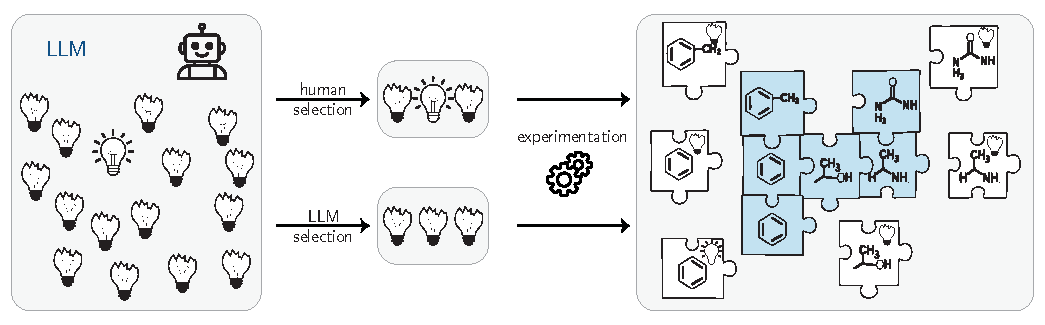
\includegraphics[width=1\textwidth]{figures/rescaled_figures/chemrev_figure13.pdf}
    \caption{\textbf{Overview of \gls{llm}-based hypothesis generation}. 
    Current methods are based on \gls{llm}-sampling methods in which an \gls{llm} proposes new hypotheses. 
    The generated hypotheses are evaluated in terms of novelty and impact either by another \gls{llm} or by a human. Then, through experimentation, the hypotheses are transformed into results which showcase that current \glspl{llm} cannot produce groundbreaking ideas, limited to their training corpus, resulting in the best cases, in incremental work. This is shown metaphorically with the puzzle. The \enquote{pieces of chemical knowledge} based on the hypothesis produced by \glspl{llm} are already present in the \enquote{chemistry puzzle}, not unveiling new parts of it.}
    \label{fig:hypothesis-generation}
\end{figure}

\subsubsection{Are LLMs Actually Capable of Novel Hypothesis Generation?}

Automatic hypothesis generation is often regarded as the Holy Grail of automating the scientific process \autocite{coley2020autonomous}. However, achieving this milestone remains challenging, as generating novel and impactful ideas requires questioning current scientific paradigms \autocite{Kuhn1962Structure}---a skill typically refined through years of experience---which is currently impossible for most \gls{ml} systems.

Current progress in \gls{ml} illustrates these limitations \autocite{kon2025exp0bench0, gu2024interesting}. Although some studies claim success in \gls{ai}-generated ideas accepted at workshops in \gls{ml} conferences via double-blind review \autocite{zhou2025tempest0}, these achievements are limited. 
First, accepted submissions often focus on coding tasks, one of the strongest domains for \glspl{llm}. Second, workshop acceptances are less competitive than main conferences, as they prioritize early-stage ideas over rigorously validated contributions. 
In chemistry, despite some works showing promise on these systems \autocite{yang2025moose0chem20}, \glspl{llm} struggle to propose functional hypotheses \autocite{si2025ideation1execution}.
Their apparent success often hinges on extensive sampling and iterative refinement, rather than genuine conceptual innovation.

As \textcite{Kuhn1962Structure} argued, generating groundbreaking ideas demands challenging prevailing paradigms---a capability missing in current \gls{ml} models (they are trained to make the existing paradigm more likely in training rather than questioning their training data), as shown in \Cref{fig:hypothesis-generation}. 
Thus, while accidental discoveries can arise from non-programmed events (e.g., Fleming’s identification of penicillin \autocite{Fleming1929antibacterial, Fleming1945penicillin}), transformative scientific advances typically originate from deliberate critique of existing knowledge \autocite{popper1959logic, Lakatos1970falsification}. In addition, very often breakthroughs can also not be achieved by optimizing for a simple metric---as we often do not fully understand the problem and, hence, cannot design a metric.\autocite{stanley2015greatness}
Despite some publications suggesting that \gls{ai} scientists already exist, such claims are supported only by narrow evaluations that yield incremental progress \autocite{novikov2025alphaevolve}, not paradigm-shifting insights. For \gls{ai} to evolve from research assistants into autonomous scientists, it must demonstrate efficacy in addressing societally consequential challenges, such as solving complex, open-ended problems at scale (e.g., \enquote{millennium} math problems
\autocite{Carlson2006millennium}).

Finally, ethical considerations become critical as hypothesis generation grows more data-driven and automated. Adherence to legal and ethical standards must guide these efforts (see \Cref{sec:safety}) \autocite{danish_gov2024hypothesis}.

With a hypothesis in hand, the next step is often to run an experiment to test it. 


\subsection{Experiment Planning}
\label{sec:planning}
Before a human or robot can execute any experiments, a plan must be created. 
Planning can be formalized as the process of decomposing a high-level task into a structured sequence of actionable steps aimed at achieving a specific goal. 
The term planning is often confused with scheduling and \gls{rl}, which are closely related but distinct concepts. Scheduling is a more specific process focused on the timing and sequence of tasks. 
It ensures that resources are efficiently allocated, experiments are conducted in an optimal order, and constraints (such as lab availability, time, and equipment) are respected.\autocite{kambhampati2023llmplanning} 
\gls{rl} is about adapting and improving plans over time based on ongoing results.\autocite{chen2022deep}

\subsubsection{Conventional Planning} 
Early experimental planning in chemistry relied on human intuition and domain expertise. 
One example of this is retrosynthesis. 
Since the 1960s, systems like \gls{lhasa} \autocite{corey1972computer} began automating retrosynthesis using hand-coded rules and heuristics\autocite{warr2014short}. 
Later tools, such as \modelname{Chematica}\autocite{grzybowski2018chematica}, expanded these efforts by integrating larger template libraries and optimization strategies. 
As reaction data grew in volume and complexity, manual rule encoding became unsustainable. 
Platforms like ASKCOS\autocite{tu2025askcos} integrated \glspl{gnn} and neural classifiers to predict reactivity and suggest conditions, enabling actionable synthetic routes. 

All applications, however, face the problem that planning is difficult because search spaces are combinatorially large and evaluating potential paths, in principle, requires a model that can perfectly predict the outcomes of different actions. Conventional approaches often rely on various forms of search algorithms such as \gls{bfs}, \gls{dfs}, \gls{mcts} \autocite{segler2017towards}. 
Those, however, are often still not efficient enough to tackle long-horizon planning for complex problems. 

\subsubsection{LLMs to Decompose Problems into Plans}
\glspl{gpm}, in particular \glspl{llm}, can potentially assist in planning with two modes of thinking. 
Deliberate (system-2-like) thinking can be used to score potential options or to decompose problems into plans. 
Intuitive (system-1-like) thinking can be used to efficiently prune search spaces. 
These two modes align with psychological frameworks known as system-1 and system-2 thinking. \autocite{kahneman2011thinking}
In the system-1 thinking, \glspl{llm} support rapid decision-making by leveraging heuristics and pattern recognition to quickly narrow down options. 
In contrast, system-2 thinking represents a slower, more analytical process, in which \glspl{llm} solve complex tasks---such as logical reasoning and planning---by explicitly generating step-by-step reasoning. \autocite{ji2025test}

Decomposing a goal into actionable milestones relies on this deliberate, system-2-style reasoning, enabling the model to evaluate alternatives and structure plans effectively. 
A variety of strategies have been proposed to improve the reasoning capabilities of \glspl{llm} during inference. 
Methods such as \gls{cot} and least-to-most prompting guide models to decompose problems into interpretable steps, improving transparency and interpretability. 
However, their effectiveness in planning is limited by error accumulation and linear thinking patterns.\autocite{stechly2024chain}
To address these limitations, recent test-time strategies such as repeat sampling and tree search have been proposed to enhance planning capabilities in \glspl{llm}. 
Repeated sampling allows the model to generate multiple candidate reasoning paths, encouraging diversity in thought and increasing the chances of discovering effective subgoal decompositions. \autocite{wang2024planning}
Meanwhile, tree search methods like \gls{tot} and \gls{rap} treat reasoning as a structured search, also using algorithms like \gls{mcts} to explore and evaluate multiple solution paths, facilitating more global and strategic decision-making. \autocite{hao2023reasoning}

Beyond purely linguistic reasoning, \glspl{llm} have also been used to interpret natural-language queries and to translate them into structured planning steps, as demonstrated by systems like \gls{llm}+P\autocite{liu2023llm} and \gls{llm}-DP\autocite{dagan2023dynamic}, which integrated \glspl{llm} with classical planners to convert planning problems into \gls{pddl}.
\glspl{llm} have also been applied to generate structured procedures from limited observations. For example, in quantum physics, a model was trained to infer reusable experimental templates from measurement data, producing Python code that generalized across system sizes. \autocite{arlt2024meta0designing} This demonstrates how \glspl{llm} can support scientific planning by synthesizing high-level protocols from low-level evidence, moving beyond symbolic reasoning to executable plan generation.

\subsubsection{Pruning of Search Spaces}

Pruning refers to the process of eliminating unlikely or suboptimal options during the search to reduce the computational burden.
Because the number of potential pathways can grow exponentially, exhaustive search may be computationally intensive. 
Classical planners employ heuristics, value functions, or logical filters to perform pruning\autocite{bonet2012action}. 
\glspl{llm} can emulate pruning through learned heuristics, intuitive judgment, or context-driven evaluation, \autocite{gao2025synergizing} reflecting system-1 thinking.
\Cref{fig:planning} illustrates how \glspl{llm} can support experimental planning by selectively pruning options.
Rule-based heuristics derived from domain knowledge can automatically discard routes involving unfavorable motifs, such as chemically strained rings or complex aromatic scaffolds. 
Meanwhile, \glspl{llm} can emulate an expert chemist's intuition by discarding synthetic routes that appear unnecessarily long, inefficient, or mechanistically implausible. 

To further enhance planning efficacy, \glspl{llm} can be augmented with external tools that estimate the feasibility or performance of candidate plans, enabling targeted pruning of the search space before costly execution. 
In \modelname{ChemCrow}, the \gls{llm} collaborated with specialized chemical tools with knowledge about molecular and reaction properites. While \modelname{ChemCrow} does not explicitly generate and prune a large pool of candidate plans, these tools serve as real-time evaluators that help the model avoid unfeasible or inefficient directions during synthesis or reaction planning.

In addition to external tools, \glspl{llm} can also engage in self-correction, a reflective strategy that identifies and prunes flawed reasoning steps within their own outputs. 
This introspective pruning supports more robust and coherent planning by discarding faulty intermediate steps before they affect final decisions. 
As such, self-correction offers a lightweight yet effective mechanism for narrowing the solution space in complex reasoning tasks. 
At the highest level of oversight, human-in-the-loop frameworks introduce expert feedback to guide pruning decisions. 
The \modelname{ORGANA} system\autocite{darvish2025organa} integrated chemist feedback into the planning process, helping define goals, resolve ambiguities, and eliminate invalid directions.
\begin{figure}[!htbp]
    \centering
        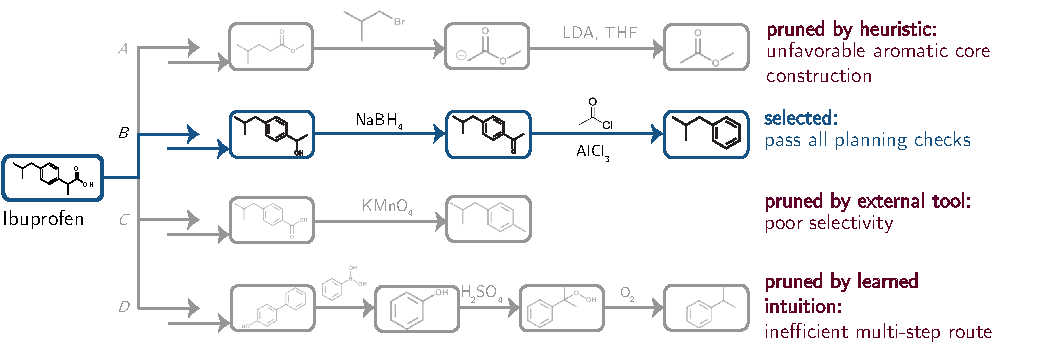
\includegraphics[width=1\textwidth]{figures/rescaled_figures/chemrev_figure14.pdf}
    \caption{\textbf{\gls{gpm}-guided retrosynthesis route planning and pruning}. \glspl{gpm} can systematically evaluate and prune retrosynthetic routes using multiple reasoning capabilities to discriminate between viable and problematic approaches. The partially overlapping arrows at the start of each route indicate multiple steps. \textbf{Route A}: This route was pruned by heuristic reasoning due to the unfavorable aromatic core construction.
    \textbf{Route B}: This route was selected as it successfully passes all \gls{gpm} planning checks, demonstrating optimal synthetic feasibility.
    \textbf{Route C}: This pathway was pruned by external tools due to the poor region-selectivity of the oxidation step.
    \textbf{Route D}: This route was pruned based on learned intuition, as it represents an inefficient multistep pathway; the route could just start with phenol instead of synthesizing it.
}
    \label{fig:planning}
\end{figure}

\subsubsection{Evaluation}
While pruning accelerates planning, its effectiveness depends on reliable evaluation---the ability to judge whether a candidate plan is valid or promising. 
However, evaluating planning quality is particularly challenging in scientific fields such as chemistry and biology. 
Many alternative plans may achieve the same goal, so evaluation is inherently ambiguous in the absence of a comprehensive world model.
In open-ended domains, evaluation is often conducted manually. 
For example, \modelname{ChemCrow} \autocite{bran2024augmenting} relied on expert review to assess the correctness and plausibility of generated outputs. 
More dynamic evaluations can be performed in simulated or real embodied environments \autocite{song2023llm, choi2024lota}, offering interactive feedback on feasibility. 
In parallel, automatic evaluation methods are emerging. 
For example, \modelname{BioPlanner}\autocite{o2023bioplanner}
used pseudocode-based evaluation, comparing \gls{llm}-generated protocols to expert-written pseudocode representations to assess plausibility and correctness without requiring manual review or physical execution.


\subsection{Experiment Execution}
Once an experimental plan is available, whether from a human scientist's idea or a sophisticated AI model, the next step is to execute it. 
Regardless of its source, the plan must be translated into concrete, low-level actions for execution. One of the main challenges of lab automation is to convert the high-level and abstract experimental plan into real-world operations carried out by the experimental hardware (liquid-handing systems, robotic arms, instruments, etc.). 

It is worth noting that, despite their methodological differences, executing experiments \textit{in silico} (running simulations or code) and \textit{in vitro} are not fundamentally different---both follow an essentially identical workflow: Plan $\rightarrow$ Instructions $\rightarrow$ Execution $\rightarrow$ Analysis. 
In a computer simulation, a researcher writes a program (plan), which is then compiled or interpreted into machine code (instructions) for the \gls{cpu}, executed to produce data, and finally the outputs are analyzed. 
In an automated laboratory, the scientist specifies a protocol (plan), which must be translated into instrument commands (instructions), executed on a robotic platform, followed by the analysis of sensor data or assay results. Both scenarios require careful translation of abstract steps into concrete actions, as well as further decision-making based on the acquired results.

The execution of \textit{in silico} experiments can be reduced to two essential steps: preparing input files and running the computational code; \glspl{gpm} can be used in both steps.\autocite{Liu2025ASA, Mendible‑Barreto2025DynaMate, Zou2025ElAgente, Campbell2025MDCrow} \textcite{Jacobs2025orca} found that using a combination of fine-tuning, \gls{cot} and \gls{rag} (see \Cref{sec:model_adaptation}) can improve the performance of \glspl{llm} in generating executable input files for the quantum chemistry software \emph{ORCA}\autocite{ORCA5}, while \textcite{Gadde2025chatbot} created \modelname{AutosolvateWeb}, an \gls{llm}-based platform that assists users in preparing input files for \gls{qmmm} simulations of explicitly solvated molecules and running them on a remote computer. 
Examples of \gls{gpm}-based autonomous agents (see 
\Cref{sec:agents}) capable of performing the entire computational workflow (i.e., preparing inputs, executing the code, and analyzing the results) are \modelname{MDCrow} \autocite{Campbell2025MDCrow} (for molecular dynamics) and \modelname{El Agente Q} \autocite{Zou2025ElAgente} (for quantum chemistry).

\Glspl{gpm} can also assist in automating \textit{in vitro} experiments. 
We can draw parallels from programming language paradigms---compiled vs.\ interpreted (see \Cref{fig:exec}A)---to better understand how \glspl{gpm} can be useful in different approaches of experiment automation. 
In compiled languages (like \modelname{C++} or \modelname{Fortran}), the entire code is converted ahead of time by another program called the \enquote{compiler} into binary machine code, which is directly executable by the hardware. 
In interpreted languages (like \modelname{Python} or \modelname{JavaScript}), a program called the \enquote{interpreter} reads the instructions line-by-line during runtime, translating and executing them on the fly. 
Compiled languages offer high performance and early error detection, making them ideal for performance-critical systems, but they require a separate compilation step and are less flexible during development. 
Interpreted languages are easier to use, debug, and modify on the fly, which makes them great for rapid development and scripting, but they generally run slower and catch errors only at runtime. 
Similarly, we can broadly categorize different approaches to experiment automation into two different groups: \enquote{compiled automation} and \enquote{interpreted automation} (see \Cref{fig:exec}B). In the compiled approach, the entire protocol is translated---either by a human or a \gls{gpm}---to low-level instructions before execution, while in interpreted automation, the \gls{gpm} plays a central role, acting as the \enquote{interpreter} and executing the protocol step by step. 
As we show below, it can be instructive to use this perspective when discussing approaches to automate experiment execution with \glspl{gpm}.


\begin{figure}[p]
    \centering
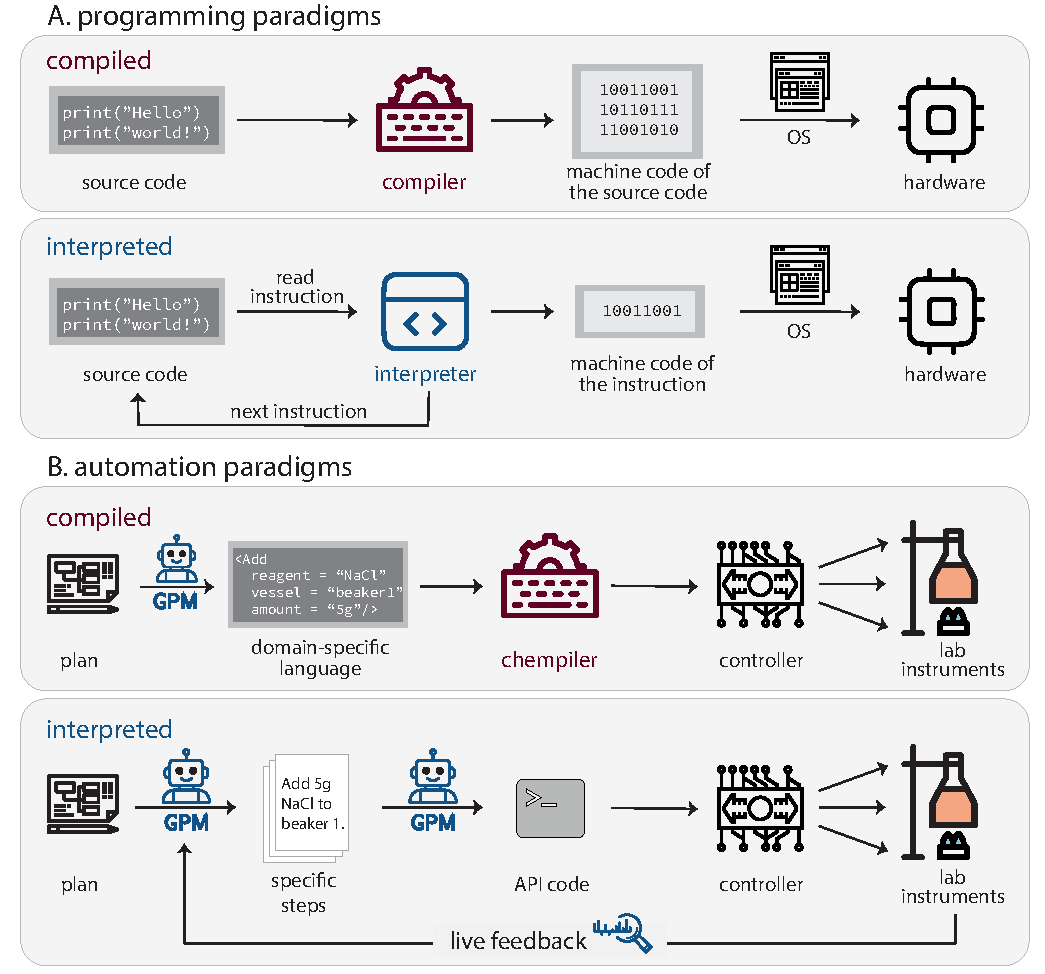
\includegraphics[width=\textwidth]{figures/rescaled_figures/chemrev_figure15+16.pdf}
    \caption{\textbf{Programming languages vs.\ lab automation. A) programming paradigms}: In compiled languages, the entire source code is translated ahead of time to machine code by the compiler. This stand-alone code is then given to the \gls{os}, which is responsible for scheduling and distributing tasks to the hardware. In interpreted languages, the interpreter reads and translates each line of the source code to machine code and hands it to the \gls{os} for execution. \textbf{B) automation paradigms}: In the compiled approach, a \gls{gpm} formalizes the protocol, a compiler, such as the chempiler\autocite{steiner2019organic}, translates the formalized protocol to hardware-specific low-level steps, which the controller then executes---a central hub tasked with scheduling and distributing commands to chemical hardware. In the interpreted approach, a \gls{gpm}, acting as the interpreter, first breaks down the protocol into specific steps, then sends them (via an \gls{api}) for execution one by one. The strength of interpreted systems is dynamic feedback: after the execution of each step, the \gls{gpm} receives a signal (e.g., data, errors), which can influence its behavior for the next steps.}
    \label{fig:exec}
\end{figure}

\subsubsection{Compiled Automation}
In the case of \enquote{compiled automation}, the experiment protocol needs to be formalized in a high-level or \gls{dsl} that describes exactly what operations to perform in what order. 
A chemical compiler (or \enquote{chempiler} \autocite{steiner2019organic}) then converts this high-level protocol into low-level code for the specific lab hardware, which is then executed by robotic instruments, orchestrated by a controller (refer to the caption of \Cref{fig:exec}B). 

\paragraph{Protocol Languages} While \modelname{Python}-based scripts are frequently used as the \textit{de facto} protocol language due to \modelname{Python}'s accessibility and flexibility,\autocite{pylabrobot,vriza2023polybot, wang2025polybot} specialized languages (\glspl{dsl}) have also been developed to provide more structured and semantically rich representations of experimental procedures.\autocite{wang2022ulsa, ananthanarayanan2010biocoder, autoprotocol2023, Park2023CMDL} 
One of the prominent examples of such languages is \gls{chidl}\autocite{xdl2023spec}, developed as part of the Chemputer architecture \autocite{steiner2019organic, mehr2020universal, hammer2021chemputation}. 
\gls{chidl} uses a \gls{json}-like format, and the experimental protocol is described by defining \modelname{Reagents}, \modelname{Vessels}, etc, and using abstract chemical commands such as \modelname{Add}, \modelname{Stir}, \modelname{Filter}, etc. 
In the next step, the \modelname{Chempiler} software takes this \gls{chidl} script and a description of the physical connectivity and composition of the automated platform as a graph and translates it into \gls{chasm} which is specific to the platform (akin to machine code). 
In practice, \gls{chidl}  has been used to automate multi-step organic syntheses with yields comparable to manual experiments.\autocite{mehr2020universal}  

Developing experimental protocols in a formal language is a non-trivial task, often requiring specialized coding expertise. 
Within the compiled approach, the role of the \gls{gpm} is to translate natural-language protocols into their formalized, machine-readable counterparts.\autocite{Lamas2024DSLXpert, jiang2024protocode, conrad2025lowering, inagaki2023robotic} \textcite{Vaucher2020AutoExtraction} used an encoder-decoder transformer model to convert English experimental procedures to structured sequences of pre-defined synthesis actions (e.g., \modelname{MakeSolution}, \modelname{SetTemperature}, \modelname{Extract}). They pre-trained the model on $2$M sentence-action pairs extracted by a rule-based \gls{nlp} algorithm and then fine-tuned it on manually annotated samples to improve accuracy. 
The model achieved exact sentence-pair matching in $61\%$ of the test samples and had more than $75\%$ overlap in $82\%$ of them. 
Although this approach accelerates automated protocol extraction from chemical literature, the output format is not directly suitable for execution. 

\textcite{Pagel2024LLMChemputer} introduced a multi-agent workflow (based on \modelname{GPT-4}) that can address this issue and convert unstructured chemistry papers into executable code. 
The first agent extracts all synthesis-relevant text, including supporting information; a procedure agent then sanitizes the data and tries to fill the gaps from chemical databases (using \gls{rag}); another agent translates procedures into \gls{chidl} and simulates them on virtual hardware; finally, a critique agent cross-checks the translation and fixes errors.

The example above shows one of the strengths of the compiled approach: it allows for pre-validation. 
The protocol can be simulated or checked for any errors before running on the actual hardware, ensuring safety. 
Another example of \gls{llm}-based validators for chemistry protocols is \modelname{CLAIRify}.\autocite{Yoshikawa2023CLAIRify} 
Leveraging an iterative prompting strategy, it uses \modelname{GPT‑3.5} to first translate the natural-language protocol into \gls{chidl} script, then automatically verifies its syntax and structure, identifies any errors, appends those errors to the prompt, and prompts the \gls{llm} again---iterating this process until a valid \gls{chidl} script is produced. 

Similar to how compiled software can be recompiled for different platforms, compiled automation is hardware-agnostic: by using appropriate compilation, a well-defined protocol can---at least in principle---be run on different robotic systems as long as they have the required capabilities.\autocite{rauschen2024universal, strieth-kalthoff2024delocalized,wilbraham2021chemPU} 
In practice, however, inconsistencies in hardware interfaces and software standards across the lab automation community make cross-platform execution challenging.

The main limitations of compiled approaches are the flip side of their strengths: low flexibility and adaptability. 
Any logic or decision-making must either be explicitly encoded within the protocol---necessitating meticulous scripting---or delegated to an external control layer.\autocite{mehr2023digitizing,leonov2024integrated} 
If something unexpected occurs (a pump clogging, a reaction taking longer than expected), the pre-compiled protocol cannot easily adjust in real-time, and human intervention or a complete recompile might be needed.

\subsubsection{Interpreted Automation}
Interpreted programming languages support higher levels of abstraction, enabling the use of more general and flexible command structures. 
Similarly, since \glspl{gpm} can translate high-level goals into concrete steps\autocite{ahn2022can, huang2022language}, they can act as an \enquote{interpreter} between the experimental intent and lab hardware. 
For instance, given an instruction \enquote{titrate the solution until it turns purple}, a \gls{gpm} agent (see \Cref{sec:agents}) can break it down into smaller steps and convert each step to executable code, allowing it to perform incremental additions of titrant and read a color sensor, looping until the condition is met. 
This conversion of concrete steps to code happens at runtime; it is not pre-compiled. 
We refer to such systems as \enquote{interpreted automation} systems. 
In contrast to the deterministic, preplanned nature of compiled systems, interpreted architectures introduce real-time decision-making.
As each action completes, the system collects sensor data (instrument readings, spectra, error messages, etc.) which the agent analyzes and decides on the next action. This allows for dynamic branching and conditional logic during the experiment execution. 

\modelname{Coscientist} \autocite{boiko2023autonomous} is an \gls{llm}-based chemistry assistant built around \modelname{GPT-4} that can autonomously design and execute experiments. 
It can take high-level goals and call tools to write code in real-time in order to control an Opentrons OT-2 liquid-handling robot. The architecture included a web-search module, a documentation module (to read instrument manuals), a \modelname{Python} execution module (to run generated code in a sandbox), and an experiment execution module that sends code to actual lab equipment.
If an error occurred, the system would get feedback and \modelname{GPT-4} would debug its own code. \modelname{Coscientist} successfully planned and executed multistep syntheses with minimal human intervention. 
For example, it efficiently optimized a palladium cross-coupling reaction with minimal human input, outperforming a standard Bayesian optimizer baseline in finding high-yield conditions.

Another example is \modelname{ChemCrow} \autocite{bran2024augmenting}, a \modelname{GPT-4}-based agent augmented with $18$ expert-designed tools for tasks like compound lookup, spectral analysis, and retrosynthesis. \modelname{ChemCrow} can perform tasks across synthesis planning, drug discovery, and materials design by invoking external software for things like retrosynthesis, property prediction, database queries, etc. 
It planned and executed the syntheses of an insect repellent, \gls{deet}, and three different organocatalysts and even guided the discovery of a new chromophore dye. 

The interpreted paradigm is highly generalizable; in principle, the same \gls{llm} agent controlling a chemistry experiment could be re-purposed to a biology or materials experiment with minimal reprogramming because it operates at the level of intent and semantic understanding. 
However, fully autonomous labs featuring interpreted automation are still experimental themselves---ensuring their reliability and accuracy remains an open challenge. 

Despite being labeled as \enquote{autonomous,} both systems mentioned above often need prompting nudges and human correction. 
In addition, these models can replicate known procedures and use databases, but they lack an understanding of mechanisms or underlying principles. Another issue is full reproducibility and long-term experiment tracking. Since the \gls{gpm}'s response might not be deterministic, small changes in prompts can yield different results and closed-source models like \modelname{GPT-4} can change over time. 
Hallucinations remain a risk, especially in planning complex or sensitive reactions. 
In addition, allowing an agent to control hardware brings safety considerations; the flexibility of \glspl{gpm} means that they can devise unanticipated actions. Designing safety nets for these systems is an active area of research. (see \Cref{sec:safety})

\subsubsection{Hybrid Approaches}
Between the two extremes of fully compiled vs.\ fully interpreted automation lies a hybrid approach that seeks to combine the best of both paradigms: the safety and reliability of compiled protocols and the \gls{ai}-driven flexibility of interpreted systems. 

The key difference from purely interpreted systems is that during each experiment run, the plan is fixed, ensuring safety and reproducibility, but between runs, the plan can dynamically change based on the \gls{gpm}’s interpretation of results. 
Once the initial plan (ideally devised by the same \gls{gpm} in a previous step) is provided to a hybrid system, instead of reducing it to smaller steps and directly sending the instructions to a laboratory one at a time, the protocol is first formalized---i.e., it is translated to a formal machine-readable format such as \gls{chidl}. Once validated, the formalized protocol is compiled and executed. After the completion of execution, the \gls{gpm} receives the results and decides what experiment to perform next. This cycle repeats, creating an autonomous optimization or discovery loop. 

This hybrid strategy is attractive because it provides a safety net against mistakes made by the \gls{gpm} interpreter; any generated procedure must pass through a formalization and verification stage before real execution, and therefore, erroneous or hallucinated steps can be caught. For example, if the interpreter hallucinated adding \SI{1000}{\milli\liter} of a solvent but the hardware has only \SI{100}{\milli\liter} capacity, it can be flagged as an error. 



\modelname{ORGANA} \autocite{darvish2025organa} is an \gls{llm}-based robotic assistant following this hybrid paradigm. 
It allows human chemists to describe their experimental goal in natural language. The system can converse with the user to clarify ambiguous requests (the agent would ask \enquote{do you mean X or Y?} if the instructions are unclear). Once the goal is understood, it uses \modelname{CLAIRify} \autocite{Yoshikawa2023CLAIRify} to convert and validate the natural-language description of a chemistry experiment into a \gls{chidl} script, which can be executed on a compatible platform. 
In one case, \modelname{ORGANA} carried out a multistep electrochemistry procedure---polishing electrodes, running an experiment, and analyzing the data---involving 19 substeps that it coordinated in parallel. 
If an unexpected observation occurred (e.g., a solution does not change color when expected), the system can notice via image analysis and modify the plan or alert the user. 
In user studies, \modelname{ORGANA} significantly reduced the manual labor and frustration for chemists, who could offload tedious tasks and trust the agent to handle low-level decisions.

\subsubsection{Comparison and Outlook}
While compiled paradigms continue to provide the backbone for reliable automation, interpreted paradigms will drive exploratory research, where adaptability is key. 
Hybrid systems are likely to be the bridge that brings \gls{ai} into mainstream lab operations, ensuring that flexibility comes with accountability. A brief comparison of the three mentioned approaches is given in \Cref{tab:execution_comparison}.

\begin{table}[ht]
\centering
\caption{\textbf{Comparison of the Compiled, Interpreted, and Hybrid Automation Paradigms}. Each approach has its strengths and weaknesses. Compiled systems favor reliability, interpreted systems allow for more flexibility, while hybrid systems try to strike a balance. }
\begin{tabular}{lccc}
\toprule
\textbf{Feature} & \textbf{Compiled} & \textbf{Interpreted} & \textbf{Hybrid} \\
\midrule
Flexibility & \textcolor{NegativeColor}{Low} & \textcolor{PositiveColor}{High} & Medium \\
Adaptivity & \textcolor{NegativeColor}{None} & \textcolor{PositiveColor}{Real-time} & Iterative \\
Reproducibility & \textcolor{PositiveColor}{High} & Medium & \textcolor{PositiveColor}{High} \\
Safety & \textcolor{PositiveColor}{High} & \textcolor{NegativeColor}{Low} & Medium \\
Setup Overhead & Medium & \textcolor{NegativeColor}{High} & \textcolor{NegativeColor}{High} \\
Industrial Readiness & \textcolor{NegativeColor}{Low} & \textcolor{NegativeColor}{Low} & \textcolor{NegativeColor}{Low} \\
\bottomrule
\end{tabular}
\label{tab:execution_comparison}
\end{table}

While we are essentially witnessing the rise of self-driving laboratories, autonomous experimentation systems present a range of challenges.\autocite{Tom2024SDL,Seifrid2022SDL} 
First, translating high-level natural-language goals into precise laboratory actions remains difficult, as \glspl{gpm} can misinterpret ambiguous instructions, leading to invalid or unsafe procedures. 
This problem is compounded by the lack of universally adopted standards for protocol formalization; while languages like \gls{chidl} show promise, inconsistencies in abstraction, device compatibility, and community uptake limit interoperability. 
Real-time execution adds further complexity, as systems must detect and respond to failures or unexpected behaviors; however, general-purpose validation mechanisms and recovery strategies remain underdeveloped. 
Hardware integration is another bottleneck; current commercial robotic platforms are prohibitively expensive and lab environments often rely on a patchwork of instruments with proprietary interfaces, and building robust, unified control layers demands considerable engineering overhead. 
Another challenge is multi-modality in chemistry; chemists use a wide variety of data (e.g., spectra, TLC plates, SEM images). 
Without integrating these forms of output, models will be limited in their decision-making. 
Finally, ensuring reproducibility and regulatory compliance requires that every step be logged, validated, and traceable at the level required for clinical or industrial adoption (see \Cref{sec:safety}. These challenges must be addressed in tandem to move from experimental demonstrations toward reliable, scalable, and trustworthy autonomous laboratories.


\subsection{Data Analysis}
The analysis of spectroscopic and experimental data in chemistry remains a predominantly manual process. 
Even seemingly straightforward steps, such as plotting or summarizing results, demand repeated manual intervention.

One key challenge that makes automation particularly difficult is the extreme heterogeneity of chemical data sources. 
Laboratories often rely on a wide variety of instruments, some of which are decades old, rarely standardized, or unique in configuration.\autocite{jablonka2022making} 
These devices output data in incompatible, non-standardized, or poorly documented formats, each requiring specialized processing pipelines. 
Despite efforts like \modelname{JCAMP-DX} \autocite{McDonald1988standard}, standardization attempts remain scarce and have generally failed to gain widespread use. 
This diversity makes rule-based or hard-coded solutions largely infeasible, as they cannot generalize across the long tail of edge cases and exceptions found in real-world workflows.

However, this exact complexity makes data analysis in chemistry a promising candidate for \glspl{gpm}. 
They are designed to operate flexibly across diverse tasks and formats, relying on implicit knowledge captured from broad training data. 
In other domains, \textcite{narayan2022can} showed that models like \modelname{GPT-3 DaVinci} can already perform classical data processing tasks such as cleaning, transformation, and error detection through prompting alone. \textcite{kayali2023chorus} introduced \modelname{Chorus} that shows that \glspl{llm} can analyze heterogeneous tabular data without task-specific training. 
\modelname{Chorus} demonstrates that by converting tables into a standardized text format and using zero-shot prompting (i.e., prompts with no examples), \glspl{llm} can flexibly analyze tables even when they differ in structure, column names, or data types.

\begin{figure}[!ht]
    \centering
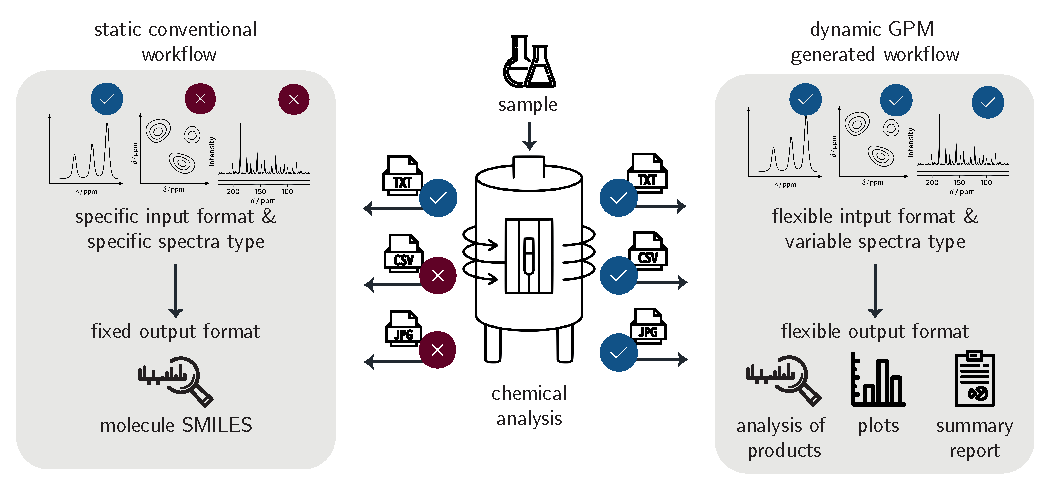
\includegraphics[width=1\textwidth]{figures/rescaled_figures/chemrev_figure17.pdf}
    \caption{\textbf{Static conventional data analysis workflow vs.\ dynamic \gls{gpm} generated workflow}. The chemical analysis can be done with a variety of possible instruments and techniques, resulting in a large number of possible output data formats. The \gls{gpm} can use these diverse, raw data and process it into easy-to-understand plots, analysis and reports. A hard-coded workflow, in contrast, is specifically made to analyze one specific data format and spectra and produces a fixed output format, e.g., the \gls{smiles} of the analyzed molecule.}
    \label{fig:anaylsis}
\end{figure}


 \subsubsection{Prompting} Initial evaluations demonstrated that \glspl{gpm} can support basic data analysis workflows. \autocite{Fu2025large} 
 For example, in chemistry, this enabled the classification of \gls{xps} signals \autocite{decurt2024large} based on peak positions, intensities, or characteristic spectral patterns).  
 
Spectroscopic data are not always available in structured textual form. 
In many practical cases, it appears as raw plots or images, making direct interpretation by \glspl{vlm} a more natural starting point for automated analysis. 
A broad assessment of \gls{vlm}-based spectral analysis was introduced with the \modelname{MaCBench} benchmark \autocite{alampara2024probing}, which systematically evaluates how \glspl{vlm} interpret experimental data in chemistry and materials science---including various types of spectra such as \gls{ir}, \gls{nmr}, and \gls{xrd}q---directly from images. They showed that while \glspl{vlm} can correctly extract isolated features from plots, the performance substantially drops in tasks requiring deeper spatial reasoning.
To overcome these limitations, \textcite{kawchak2024high} explored two-step pipelines that decouple visual perception from chemical reasoning. First, the model interprets each spectrum individually (e.g., converting  \gls{ir}, \gls{nmr}, or \gls{ms} images into textual peak descriptions), and second, a \gls{llm} analyzes these outputs to propose a molecular structure based on the molecular formula. 

\subsubsection{Agentic Systems}
Beyond zero-shot prompting of \glspl{gpm}, one can develop agentic systems that combine multiple analysis steps end-to-end. 
In this regard, \textcite{ghareeb2025robin0} developed \modelname{Robin}---a multi-agent system for assisting biological research with hypothesis generation (see \Cref{fig:hypothesis-generation}) and experimental analysis. 
The data analysis agent \modelname{Finch} performs autonomous analysis of raw or preprocessed experimental data, such as \gls{rna} sequencing and flow cytometry. 
Given a user prompt (e.g., \enquote{\gls{rna} sequencing differential expression analysis}), \modelname{Finch} executes code in a Jupyter notebook to process the data, apply relevant statistical methods, and generate interpretable outputs. For flow cytometry, this includes gating strategies and significance testing, while for \gls{rna} sequencing, it encompasses differential expression and gene ontology enrichment analysis. 
Currently, only these two data types are supported, and expert-designed prompts are still required to ensure reliable results. 

Recent work extends agentic systems beyond single-step data evaluation toward executing and optimizing entire workflows. \textcite{mandal2024autonomous} introduced \modelname{AILA} (Artificially Intelligent
Lab Assistant) utilizing \gls{llm}-agents to plan, code, execute, and revise complete \gls{afm} analysis pipelines. 
The system handles tasks such as image processing, defect detection, clustering, and extraction of physical parameters. 
Compared to systems like \modelname{Finch}, \modelname{AILA} shifts the focus from generating summaries to performing and improving full experimental analyses with minimal user input while maintaining transparency and reproducibility through code and reports.

\subsubsection{Current Limitations}
While \glspl{gpm} offer promising capabilities for automating scientific data analysis, several limitations remain. 
Recent evaluations such as \modelname{FMs4Code} \autocite{tian2024scicode} have shown that even state-of-the-art models like \modelname{GPT-4-Turbo} and \modelname{Claude 2} frequently produce syntactically correct but semantically incorrect code when tasked with common data analysis steps, such as reading files, applying filters, or generating plots. 
Typical issues include incorrect column usage, or inconsistent output formatting.

These technical shortcomings are reinforced by the model's sensitivity to prompt formulation. As demonstrated by \textcite{Yan2020auto} and \textcite{alampara2024probing}, minor changes in wording or structure can lead to significantly different outputs, highlighting a lack of robustness in prompt-based control. 

Together, these findings suggest that while foundation models can generalize across diverse data formats and analysis types, their current performance is not yet sufficient for fully autonomous use in scientific analysis settings. 
Robust prompting strategies, post-generation validation, and human oversight remain essential components in practice.



\subsection{Reporting}
To share insights obtained from data analysis, one often converts them into scientific reports. 
Also, in this step, \glspl{gpm} can take a central role, which we discuss in the following.

Reporting refers to converting scientific results into shareable reports, scientific publications, blogs, and other forms of content. 
This section describes two main applications of \glspl{llm} in scientific reporting: converting data into explanations and the first steps towards using these models as fully-fledged writing assistants.

\subsubsection{From Data to Explanation}

The lack of explainability of \gls{ml} predictions generates skepticism among experimental chemists\autocite{wellawatte2025human}, hindering the wider adoption of such models.\autocite{wellawatte2022model}
One promising approach to address this challenge is to convey explanations of model predictions in natural language. 
An approach proposed by \textcite{wellawatte2025human} is to couple \glspl{llm} with feature importance analysis tools, such as \gls{shap} or \gls{lime}. 
In this framework, \glspl{llm} can additionally interact with tools such as \gls{rag} over \modelname{arxiv} to provide evidence-based explanations.

\subsubsection{Writing Assistance} When considering \gls{ml}-based assistance in scientific writing, we can distinguish two primary modes: systems that aid authors during the active writing process and tools that optimize or refine scientific articles after initial drafting.

The former refers to the use of writing copilots that can suggest syntax improvement, identify text redundancies,\autocite{khalifa2024using} caption figures and tables\autocite{hsu2021scicap,selivanov2023medical}, or provide caption-figure match evaluation\autocite{hsu2023gpt04}, but also more specific applications like writing alt-text (descriptive text that explains the meaning and purpose of an image in digital content)\autocite{singh2024figura11y}. 

Under the latter mode, \gls{gpm} can be used to assist non-native English speakers with scientific writing \autocite{giglio2023use}.
It could even allow authors to write in their native language and use \gls{gpm} for communicating scientific results in English.

Another application of \gls{llm} is to assist with completing checklists before submitting a publication. For example, \textcite{goldberg2024usefulness} benchmark the use of \glspl{llm} in completing the author checklist for the \gls{neurips} 2025. They concluded that $70\%$ of the authors found the \gls{llm}-assistant useful, with the same fraction indicating they would revise their own checklist based on the model feedback.




\subsubsection{Vision} 

Few have ventured into fully automating the writing process.\autocite{yamada2025ai} 
While at its inception, reporting using \gls{gpm} has tremendous potential. 
In \Cref{fig:writing_with_ml} we showcase how the future of reporting could look like if we were to integrate \gls{gpm} at each step of the process.

\begin{figure}[!ht]
    \centering
        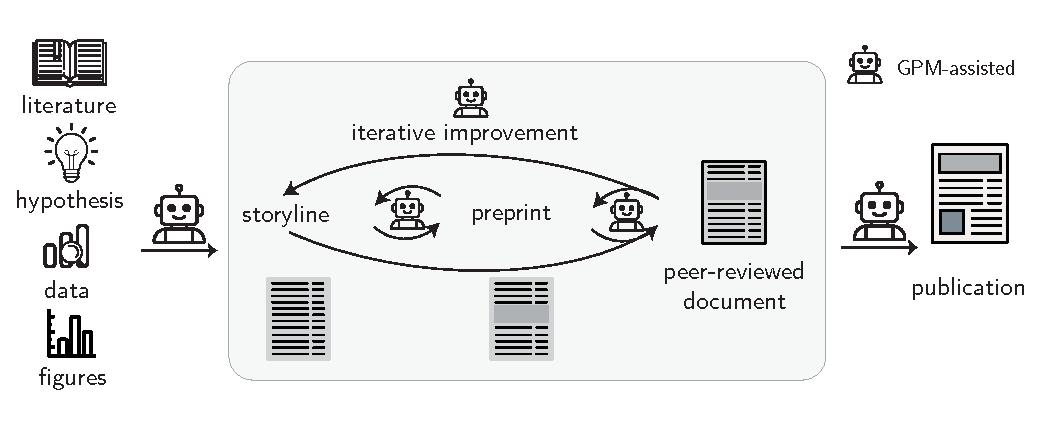
\includegraphics[width=1\textwidth]{figures/rescaled_figures/chemrev_figure18.pdf}
    \caption{\textbf{Vision for \gls{gpm} in reporting, a visualization of the scientific writing process}. \glspl{gpm} can be used at every stage of the process. For creating the pre-print, we can utilize the multimodal capabilities of these models to write detailed captions for figures. For the peer-review process, we can harness the ability of \glspl{gpm} to summarize and prioritize information (e.g., design a time-efficient plan to address the peer review). When converting a document from a peer-reviewed pre-print, we often need to implement the publisher's requirements. In this case, we can make use of agentic systems that would assist with minor text fixes or document restructuring.}
    \label{fig:writing_with_ml}
\end{figure}

An idea entertained by \textcite{li2023teach} in the context of education is personalized writing. 
However, it is still widely unexplored in its goal: to make science accessible to everyone. 
A personalized model that learns user preferences and domain expertise can be used to deliver the message of a scientific article in simpler terms. 
As a result, we might observe a rise in cross-domain scientific collaborations and a rising interest in science. 

\section{Accelerating Applications}
The application of accelerated approaches in the scientific discovery cycle (see \Cref{fig:applications}) hinges on their ability to streamline and enhance each stage of the process.
However, a fundamental challenge in effectively implementing these approaches lies in the choice of machine-readable representation.

This challenge is particularly evident in the representation of molecules and materials, which must balance computational efficiency with the preservation of structural, compositional, and functional properties. 
Take, for example, the high-temperature superconductor \ce{YBa2Cu3O_{7-x}}. 
While atomic positions and coordinates are theoretically sufficient to solve the Schrödinger equation and describe this material, such a representation may not provide the adaptability necessary for diverse tasks. What defines a good representation depends on the problem. \autocite{huang2016understanding}. 
A representation designed to predict critical temperature must efficiently encode the relationship between oxygen stoichiometry and superconducting properties, emphasizing features like oxygen vacancy patterns and charge transfer mechanisms. 
Conversely, a representation for structural stability might prioritize different geometric or bonding characteristics.

This tension has led to three primary strategies for representing molecules and materials (read \Cref{sec:common_representations} to learn in detail about the different representations that currently exist). 
First, domain-specific text-based formats---such as \gls{smiles} \autocite{weininger1988smiles}, \gls{selfies} \autocite{krenn2020self}, and \gls{cif} \autocite{hall1991crystallographic}---offer compact, machine-readable encodings of structural information. While these necessarily omit certain physical details, their computational tractability has enabled breakthroughs, as demonstrated by \textcite{jablonka2024leveraging} in their \gls{llm}-based generation of valid molecular and material structures.

Yet, the question remains: Which representation is optimal for a given task? Future advances in accelerated discovery will likely hinge on adaptive representations that dynamically balance these competing demands.

\subsection{Property Prediction} \label{sec:prediction}

\glspl{gpm} have emerged as a powerful tool for predicting molecular and material properties, offering an alternative to traditional quantum mechanical calculations or specialized \gls{ml} models. 
Current \gls{gpm}-driven property prediction tasks span both classification and regression. 
Unlike conventional approaches that rely on task-specific architectures and extensively labeled data, \glspl{gpm} have demonstrated strong generalization capabilities across diverse domains, efficiently adapting to various prediction tasks. 
Their success extends to multiple datasets, from standardized benchmarks such as \modelname{MoleculeNet} \autocite{wu2018moleculenet}, to curated datasets targeting specific applications such as antibacterial activity \autocite{chithrananda2020chemberta} or photovoltaic efficiency\autocite{aneesh2025semantic}.

Three key methodologies have been explored to adapt \glspl{llm} for property prediction: prompting techniques (see \Cref{sec:prompting}), fine-tuning (see \Cref{sec:fine-tuning}) on domain-specific data, and \gls{rag} (see \Cref{sec:rag}) approaches that combine \glspl{llm} with external knowledge bases. 

\begin{table}[htbp]
    \centering
    \caption{\textbf{Non-comprehensive list of \glspl{gpm} applied to property prediction tasks}. The table presents different models and their applications across different molecular and materials property prediction benchmarks, showing the diversity of properties (from molecular toxicology to crystal band gaps), datasets used for evaluation, modeling approaches (prompting, fine-tuning, or retrieval-augmented generation), and task types (classification or regression.)}
    \label{tab:property_prediction_models}
    \resizebox{\textwidth}{!}{%
    \begin{tabular}{lllcc}
        \toprule
        \textbf{Model} & \textbf{Property} & \textbf{Dataset} & \textbf{Approach}  & \textbf{Task}\\
        \midrule
        \multirow{7}{*}{GPT-Chem\autocite{jablonka2024leveraging}} & HOMO/LUMO & QMUGs\autocite{isert_qmugs_2022} & \multirow{7}{*}{FT} & C, R \\
        & Solubility & DLS-100\autocite{mitchell_dls-100_2017} & & C, R \\
        & Lipophilicity & LipoData\autocite{jablonka2024leveraging} & & C, R \\
        & Hydration Free Energy & FreeSolv\autocite{mobley_freesolv_2014} & & C, R \\
        & Photoconversion Efficiency & OPV\autocite{jablonka2024leveraging} & & C, R  \\
        & Toxicology & Tox21\autocite{richard_tox21_2021} & & C, R  \\
        & $\text{CO}_2$ Henry Coefficients of MOFs & MOFSorb-H\autocite{lin_silico_2012} & & C, R \\
        \cmidrule{1-5}
        \multirow{3}{*}{LLM-Prop\autocite{rubungo_llm-prop_2023}} & Band Gap & \multirow{3}{*}{CrystalFeatures-MP2022\autocite{rubungo_llm-prop_2023}} & \multirow{3}{*}{P} &  R  \\
        & Volume & & & R \\
        & Is the band gap direct?&  & & C \\
        \midrule
        \multirow{12}{*}{LLM4SD\autocite{zheng2025large}} & Blood-brain barrier penetration & BBBP\autocite{sakiyama_prediction_2021} & \multirow{10}{*}{P} & C \\
        & FDA approval & ClinTox\autocite{wu2018moleculenet} & & C \\
        & Toxicology & Tox21\autocite{richard_tox21_2021} & & C \\
        & Drug-related side effects & SIDER\autocite{kuhn_sider_2016} & & C \\
        & HIV replication inhibition & HIV\autocite{wu2018moleculenet} & & C \\
        & $\beta$-secretase binding & BACE\autocite{wu2018moleculenet} & & C \\
        & Solubility & ESOL\autocite{wu2018moleculenet} & & R \\
        & Hydration Free Energy & FreeSolv\autocite{mobley_freesolv_2014} & & R \\
        & Lipophilicity & Lipophilicity\autocite{wu2018moleculenet} & & R \\
        & Quantum Mechanics & QM9\autocite{wu2018moleculenet} & & R \\
        \midrule
        \multirow{4}{*}{\modelname{LLaMP\autocite{chiang2024llamp}}} & Bulk modulus & \multirow{4}{*}{Materials Project\autocite{riebesell2025framework}} & \multirow{4}{*}{RAG} & R \\
        & Formation energy & & & R \\
        & Electronic bandgap & & & R \\
        & Multi-element electronic bandgap & & & R \\
        \bottomrule
    \end{tabular}
    }
    \vspace{0.5em}
    \footnotesize
    \begin{minipage}{\linewidth}
        \textbf{Key:}  P = prompting; FT = fine-tuned model; RAG = retrieval-augmented generation; C = Classification; R = Regression
    \end{minipage}
\end{table}

\subsubsection{Prompting} 
Prompt engineering involves designing targeted instructions to guide \glspl{gpm} in performing specialized tasks without altering their underlying parameters by leveraging their embedded knowledge. 
In molecular and materials science, this strategy goes beyond simply asking a model to predict properties. 
It also includes carefully structured prompts to elicit detailed molecular and material descriptions directly from the model's pre-trained knowledge.

\textcite{liu2025integrating} conducted a comprehensive evaluation of different prompting techniques to predict the properties of organic small molecules and crystal materials. 
Some of these techniques included domain-knowledge (prior knowledge was embedded in the prompt), expert (role-play instructions), and few-shot \gls{cot} (the text\textit{\enquote{Let's think step by step}} is added) prompting. 
Of these, domain knowledge achieved maximum performance. However, their evaluation was limited to a relatively small set of molecules and tasks, and the effectiveness of their domain-knowledge approach may not generalize to other molecular property domains.

Building on these foundational prompting strategies, few-shot prompting approaches leverage \gls{icl} to enhance performance through selected examples \textcite{liu2024moleculargpt} used \gls{smiles} string representations of molecules with few-shot \gls{icl}, retrieving structurally similar molecules as demonstrations to enhance property prediction. 
This approach highlights how \gls{icl} can transfer knowledge from similar molecule examples without requiring model fine-tuning for each task. 
However, the effectiveness of \gls{icl} depends on the quality of retrieved examples.

\textcite{fifty2023incontext} moved beyond direct text prompting of molecules and introduced \gls{camp}: an \gls{icl} algorithm that uses a two-stage encoding approach without relying on pre-trained \glspl{llm}.
First, a specialized \gls{mpnn} encodes molecule graphs into molecular embeddings rather than processing them as raw text. 
These embeddings are then fed into a transformer encoder, which learns contextualized representations across the support set (a small collection of labeled molecule-property pairs) and the unlabeled query molecules. They demonstrated \gls{camp}'s ability to outperform existing few-shot learning baselines by providing relevant molecular examples within the prompt context. However, this approach is constrained by the context-length limitations of the underlying \glspl{lm} and the challenge of selecting optimal demonstration examples.

More sophisticated approaches have leveraged prompting as part of multi-modal frameworks. The \modelname{LLM4SD} pipeline by \textcite{zheng2025large} employs specialized prompts to guide \glspl{lm} through their pre-trained knowledge on scientific literature, generating known rules (e.g., molecules weighing under \SI{500}{Da} are more likely to pass the blood-brain barrier) that transform molecules into feature vectors (e.g. \ce{CCO} could translate to a vector $[2,46.07,1,1]$ where each number represents a feature of the molecule, in this example [\# \ce{C}, MW, \# \ce{H}-bond donors, \# \ce{H}-bond acceptors]) for use with a random forest model, which they consider \enquote{interpretable}. 
This approach outperformed specialized \gls{sota} models across $58$ benchmark tasks, while providing interpretable reasoning about prediction logic (see \Cref{tab:property_prediction_models} for properties predicted by this model). However, its reliance on rule extraction may limit its ability to capture complex, non-linear relationships that specialized deep learning models can identify.

\paragraph{\glspl{llm} as Feature Extractors} Another emerging application of \glspl{llm} is their use as \enquote{feature extractors}, where they generate textual or embedded representations of molecules or materials. For instance, in materials science, \textcite{aneesh2025semantic} employed \glspl{llm} to generate text embeddings of perovskite solar cell compositions. 
These embeddings were subsequently used to train a \gls{gnn} for predicting power conversion efficiency, demonstrating the potential of \glspl{llm} to enhance feature representation in materials informatics. 
Similarly, in the molecular domain, \textcite{srinivas2024crossmodal} used zero-shot \gls{llm} prompting (see \Cref{box: cot_prompting} for prompt examples) to generate detailed textual descriptions of molecular functional groups, which are used to train a small \gls{lm}. This \gls{lm} is used to compute text-level embeddings of molecules. Simultaneously, they generate molecular graph-level embeddings from \gls{smiles} string molecular graph inputs. They finally integrate the graph and text-level embeddings to produce a semantically enriched embedding.
\begin{promptbox}\label{box: cot_prompting}
    \textbf{\gls{cot} Prompting}\autocite{srinivas2024crossmodal}\\
    Prompt 1: What is the molecular structure of this chemical \gls{smiles} string? Could you describe its atoms, bonds, functional groups, and overall arrangement? \\
    Prompt 2: What are the physical properties of this molecule, such as its boiling point and melting point?\\
    ...\\
    Prompt 14: Are there any environmental impacts associated with the production, use, or disposal of this molecule?
\end{promptbox}
In a different implementation of fine-tuning, \textcite{balaji2023gptmolberta} used \modelname{ChatGPT} to generate text descriptions of molecules that were then used to train a \modelname{RoBERTa} (125M) model for property prediction, showing how \gls{lm}-generated representations can access latent spaces that \gls{smiles} strings alone might not capture.
Similarly, \textcite{li2024unveiling} introduced the \modelname{MoleX} framework, which fine-tunes \modelname{ChemBERTa-2}\autocite{ahmad2022chemberta} on Group \gls{selfies} \autocite{cheng2023group} (a functional group-based molecular representation) to then extract a single \gls{llm}-derived embedding of molecules that captures the chemical semantics at the functional group level. This allowed them to determine which functional groups or fragments contribute to molecular properties, which in turn can be converted into reliable explanations of said properties.

\subsubsection{Fine-Tuning}\label{sec:prediction_FT}
\begin{figure}[htb] 
    \centering
    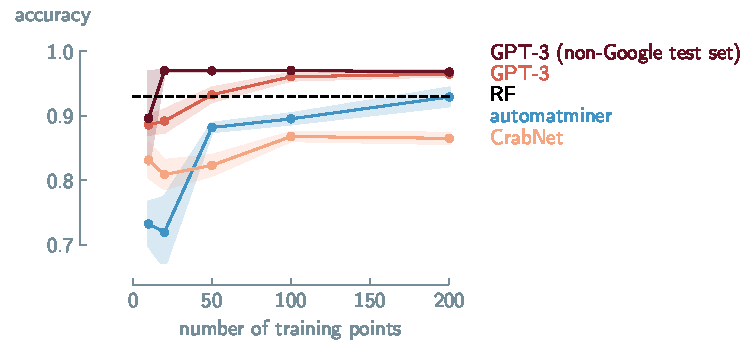
\includegraphics[width=1\textwidth]{figures/property_gptchem.pdf}
    \caption{\textbf{Fine-tuned \modelname{GPT-3} for predicting solid-solution formation in high-entropy alloys} Performance comparison of different \gls{ml} approaches as a function of the number of training points. Results are shown for \modelname{Automatminer} (blue), \modelname{CrabNet} transformer (orange),  fine-tuned \modelname{GPT-3} (red), with error bars showing standard error of the mean. The non-Google test set shows the fine-tuned \modelname{GPT-3} model tested on compounds without an exact Google search match (dark red). The dashed line shows performance using random forest. \modelname{GPT-3} achieves comparable accuracy to traditional approaches with significantly fewer training examples. Data adapted from \textcite{jablonka2024leveraging}}
    \label{fig:gptchem}
\end{figure}

\paragraph{\gls{lift}} \textcite{dinh2022lift} showed that reformulating regression and classification as \gls{qa} tasks enables the use of unmodified model architecture while improving performance (see \Cref{sec:fine-tuning} for a deeper discussion of \gls{lift}). 
In recognizing the scarcity of experimental data and acknowledging the persistence of this limitation, \textcite{jablonka2024leveraging} designed a \gls{lift}-based framework using \modelname{GPT-3} fine-tuned on task-specific small datasets (see \Cref{tab:property_prediction_models}). 
They seminally demonstrated that fine-tuned \modelname{GPT-3} can match or surpass specialized \gls{ml} models in various chemistry tasks. A key finding was fine-tuned \modelname{GPT-3}'s ability to generalize beyond training data. 
When tested on compounds absent from Google Search (and likely its training data), it performed well, proving that it was not simply recalling memorized information (see \Cref{fig:gptchem}).

In a follow-up to \textcite{jablonka2024leveraging}'s work, \textcite{vanherck2025assessment} systematically evaluated this approach across 22 diverse real-world chemistry case studies using three open-source models. They demonstrate that fine-tuned \glspl{llm} can effectively predict various material properties. For example, they achieved $96\%$ accuracy in predicting the adhesive free-energy of polymers, outperforming traditional \gls{ml} methods like random forest ($90\%$ accuracy). When predicting properties of monomers using \gls{smiles} notation, the fine-tuned models reached average accuracies of $84\%$ across four different properties. Particularly notable was the ability of \glspl{llm} to work with non-standard inputs, like in a protein phase separation study they did, where raw protein sequences could be directly input without pre-processing and achieve $95\%$ prediction accuracy. At the same time, when training datasets were very small (15 data points), the predictive accuracy of all fine-tuned models was lower than the random baseline (e.g. MOF synthesis). These case studies preliminarily demonstrate that these models can achieve predictive performance with some small datasets, work with various chemical representations (\gls{smiles}, \gls{mof}id, and \gls{iupac} names), and can outperform traditional \gls{ml} approaches for some material property prediction tasks.

In the materials domain, \modelname{LLMprop} fine-tunes \modelname{T5}\autocite{raffel2020exploring} to predict crystalline material properties from text descriptions generated by \modelname{Robocrystallographer}\autocite{ganose2019robocrystallographer}. By discarding \modelname{T5}’s decoder and adding task-specific prediction heads, the approach reduces computational overhead while leveraging the model’s ability to process structured crystal descriptions. The method demonstrates that natural language representations can effectively capture key material features, offering an alternative to traditional graph-based models like \glspl{gnn}.

Fine-tuning has been used to adapt \glspl{ssm} like Mamba (see \Cref{sec:example_architectures}). By pre-training on 91 million molecules, the Mamba-based model \modelname{$\text{O}_{SMI}-{\text{SSM}-}336\textit{M}$} outperformed transformer methods (\modelname{Yield-BERT}\autocite{krzyzanowski2025exploring}) in reaction yield prediction (e.g., Buchwald-Hartwig cross-coupling) and achieved competitive results in molecular property prediction benchmarks.\autocite{soares2025mamba-based} 

\paragraph{Foundational \glspl{gnn} and \glspl{mlip}} The fine-tuning approach has been applied to \enquote{foundational \glspl{gnn}} \autocite{sypetkowski2024scalability, shoghi2023molecules} and \glspl{mlip}, approaches distinct from \glspl{gpm}. For example, \textcite{shoghi2023molecules, sypetkowski2024scalability} show \gls{sota} performance on property prediction tasks.
\enquote{Foundational} \glspl{mlip} pre-trained on large datasets encompassing many chemical elements can be fine-tuned for specific downstream tasks \autocite{batatia2022mace}, such as calculating sublimation enthalpies of molecular crystal polymorphs \autocite{kaur2025data}.

\paragraph{Limitations} One central challenge is finding balance in datasets. In practical applications, researchers often have many more examples of poor-performing materials than optimal ones, resulting in unbalanced datasets that can diminish model performance. \textcite{vanherck2025assessment} point out that in the catalyzed cleavage reaction study, only $3.8\%$ of catalysts were labeled as \enquote{good}, forcing researchers to reduce their training set significantly to maintain balance. They also note that \glspl{llm} struggle with highly complex or noisy datasets, as seen in their study of catalytic isomerization, where even after hyperparameter optimization, the models failed to achieve meaningful predictive power due to the high noise in the experimental data and limited sample size. Finally, they note that although \glspl{llm} can work with different chemical representations, the choice of representation significantly impacts performance. For example, when predicting polymerization rates, models using \gls{smiles} notation significantly outperformed those using \gls{iupac} names, indicating that representation selection remains an important consideration.

Fine-tuning effectively adapts \glspl{llm} to specialized chemistry tasks, but its dependence on static datasets hinders adaptability to new or evolving knowledge. \gls{rag}, whose fundamentals are described in detail in \Cref{sec:rag}, overcomes these limitations by dynamically integrating external data sources, enabling more flexible and up-to-date reasoning.

\subsubsection{Agents}

Caldas Ramos et al.\ introduce \modelname{MAPI-LLM}, a framework that processes natural-language queries about material properties using an \gls{llm} to decide which of the available tools such as the Materials Project \gls{api}, the Reaction-Network package, or Google Search to use to generate a response. \autocite{Jablonka2023} \modelname{MAPI-LLM} employs a \gls{react} prompt (see \Cref{sec:arch_agents} to read more about \gls{react}), to convert prompts such as  \textit{\enquote{Is $Fe_2O_3$ magnetic?}} or \textit{\enquote{What is the band gap of Mg(Fe3O3)2?}} into queries for Materials Project \gls{api}. 
The system processes multi-step prompts through logical reasoning, for example, when asked \textit{\enquote{If Mn2FeO3 is not metallic, what is its band gap?}}, the \gls{llm} system creates a two-step workflow to first verify metallicity before retrieving the band gap.

Building on this foundation of agent-based materials querying, \textcite{chiang2024llamp} advanced the approach with \modelname{LLaMP}, a framework that employs \enquote{hierarchical} \gls{react} agents to interact with computational and experimental data. This \enquote{hierarchical} framework employs a supervisor-assistant agent architecture where a complex problem is broken down and tasks are delegated to domain-specific agents.  \modelname{LLaMP} addresses the challenge of hallucinations more effectively than standard \gls{llm} approaches by grounding responses in retrieved materials databases, retrieving materials data (e.g., crystal structures, elastic tensors) while counteracting systematic \gls{llm} biases in property predictions. These biases include the tendency for \glspl{llm} to overestimate certain properties like bulk moduli and to exhibit errors in bandgap predictions based on compositional patterns learned during training rather than physical principles.


\subsubsection{Core Limitations}\label{sec:property_core_limits}

\begin{figure}[htb]
    \centering
    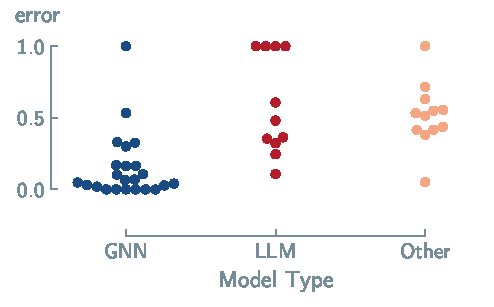
\includegraphics{figures/property_mattext.pdf}
    \caption{\textbf{Normalized error distributions for materials property prediction models across different architectures}. Each point represents the normalized error of a model on a specific property prediction task. Normalization was achieved with min/max values of each dataset to produce a range of errors between 0 and 1. The first column (blue) shows \gls{gnn} based models, the second column (red) displays \gls{llm} approaches, and the third column (orange) represents other baseline methods and \gls{sota} models including \modelname{CrabNet}. \autocite{Wang_2021} Lower values indicate better predictive performance. Data adapted from \textcite{alampara2024mattext}}
    \label{fig:property_limitations}
\end{figure}

\noindent \textcite{alampara2024mattext} introduced \modelname{MatText}, a framework for evaluating \glspl{lm} ability to predict properties of materials using text-based representations. 
Their findings indicate that current \glspl{llm} (including pre-trained \modelname{BERT} and fine-tuned \modelname{LLaMA-3-8B}) are effective for tasks relying purely on compositional information (e.g., element types and local bonding patterns), but struggle to leverage geometric or positional information encoded in text, as reflected in \Cref{fig:property_limitations}. 
This observation suggests that transformer-based architectures may be fundamentally limited to applications where spatial understanding is not required. 
Their experiments with data scaling and text representations reveal that increasing pre-training data or adding geometric details fails to improve downstream property prediction, challenging the conventional assumption that larger models and datasets universally enhance performance. \autocite{frey2023neural} 
Notably, \textcite{frey2023neural} demonstrated power-law scaling in chemical \glspl{llm}, but \modelname{MatText}'s results imply that such scaling may not overcome architectural biases against geometric reasoning in materials tasks.\autocite{gruver2024promises}

\subsection{Molecular and Material Generation} \label{sec:mol_generation}

\begin{figure}[htbp!]
    \centering
    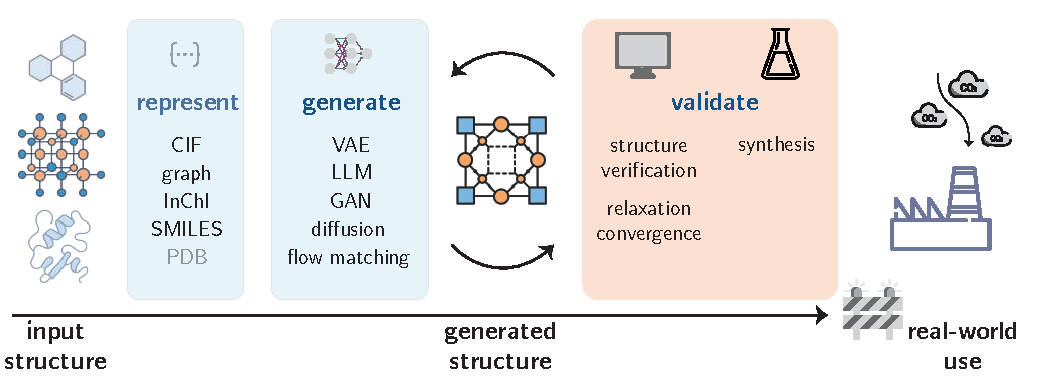
\includegraphics[width=1\textwidth]{figures/rescaled_figures/chemrev_figure21.pdf}
    \caption{\textbf{Pipeline for molecular and materials generation} The workflow begins with input structures represented in various formats, which are used to train \gls{ml} models to generate novel molecular and material structures. The generated structures should undergo a feedback loop through validation processes before being applied in the real world. Blue boxes indicate well-established areas of the pipeline with mature methodologies, while the red box represents critical bottlenecks.}
    \label{fig:generation}
\end{figure}

\noindent Early work in molecular and materials generation relied heavily on unconditional generation, where models produce novel structures without explicit guidance, relying solely on patterns learned from training data. For example, latent space sampling in autoencoders, where random vectors are decoded into new structures.\autocite{yoshikai2024novel} These methods excel at exploring chemical space broadly but lack fine-grained control. 
This limitation underscores the need for conditional generation, using explicit prompts or constraints (e.g., property targets, structural fragments), to steer \glspl{gpm} toward meaningful molecule or material designs. 
Beyond the generation step, as \Cref{fig:generation} shows, critical bottlenecks persist in synthesizability and physical consistency at the validation stage.

\subsubsection{Generation}\label{sec:generation}

\paragraph{Prompting}
While zero-shot and few-shot prompting strategies demonstrate promising flexibility for molecule generation, benchmark studies \autocite{guo2023large} reveal significant limitations that restrict their practical utility. \textcite{guo2023large} exposed fundamental gaps in \glspl{llm}' molecular design capabilities through a systematic evaluation. \modelname{GPT-4} was reported to produce chemically valid \gls{smiles} $89\%$ of the time but achieving less than $20\%$ accuracy in matching the target specifications. 
This result is far below specialized models like \modelname{MolT5}\autocite{edwards2022translation}. 
They conclude that this performance gap stems from \glspl{llm}' inadequate understanding of \gls{smiles} syntax and structure-property relationships. 
Subsequent work by \textcite{bhattacharya2024large} explored whether systematic prompt engineering could overcome these limitations, demonstrating that these prompts could guide \modelname{Claude 3 Opus} to generate chemically valid molecules ($97\%$ syntactic validity) with controlled modifications, including fine-grained structural changes (median Tanimoto similarity $0.67$--$0.69$) and predictable electronic property shifts (\SIrange{0.14}{0.27}{eV} \gls{homo} energy changes). Hybrid approaches like \modelname{FrontierX} extend this method with knowledge-augmented prompting, where \glspl{llm} generate both molecule predictions and explanations that are used to fine-tune smaller \glspl{lm}, with all resulting embeddings ultimately combined via hierarchical attention mechanisms to produce the final \gls{smiles} representation\autocite{srinivas2024crossing}. 
It showed improved accuracy over pure prompting strategies but sacrificed the generalizability that makes \glspl{llm} attractive, as the model requires re-training for each new molecular domain. 

\paragraph{Fine-Tuning} To overcome the limitations of prompting, fine-tuning has been adopted in molecular and materials generation, much like its use in property prediction with \gls{lift}-based frameworks (see \Cref{sec:fine-tuning} for a deeper explanation of \gls{lift} and \Cref{sec:prediction_FT} for a discussion of \gls{lift} applied to property prediction tasks). \textcite{yu2024llasmol} demonstrated that systematic fine-tuning in various chemical tasks including molecule generation from captions can improve performance while remaining parameter-efficient, using only $0.58\%$ of trainable parameters via \gls{lora}.

The molecule-caption translation task (\modelname{Mol2Cap}), which involves generating textual descriptions from molecular representations and vice versa (Cap2Mol), has become a standard benchmark for evaluating \glspl{gpm} for molecule generation. \autocite{edwards2022translation} Under the \enquote{Mol2Cap}/\enquote{Cap2Mol} task paradigm, \gls{icma} avoids domain-specific pre-training by combining retrieval-augmented in-context learning with fine-tuning on \gls{icl} examples.\autocite{li2025large} 
On the ChEBI-20\autocite{edwards2021text2mol} and PubChem324k\autocite{liu2023molca} datasets, \gls{icma} nearly doubles baseline performance, with \gls{icma} powered by\modelname{Mistral-7B} achieving a 0.581 \gls{bleu} score in \modelname{Mol2Cap} and $46.0\%$ exact match in \modelname{Cap2Mol}.\autocite{li2025large} 
However, its reliance on retrieved examples raises concerns about generalization to novel scaffolds. 
Similarly, \modelname{MolReFlect} enhances fine-grained alignment through a teacher-student framework, where a larger \gls{llm} (e.g., \modelname{GPT-4}) extracts substructure-aware captions to guide a smaller model (\modelname{Mistral-7B}), improving \modelname{Cap2Mol} accuracy while reducing hallucinations.\autocite{li2024molreflect} 
Meanwhile, \modelname{PEIT-LLM} extends the task to property-conditioned generation, using instructions (\gls{smiles}-text-property tuples) to optimize for captioning and prediction jointly.\autocite{lin2025property} 

Fine-tuned \glspl{lm} have shown promise in molecule and materials generation. 
However, their reliance on decoding and \gls{smiles}/\gls{selfies} representations introduces fundamental limitations: degeneracy (multiple valid \gls{smiles} for the same molecule) and difficulty capturing complex structural relationships implicit in textual descriptions.

\paragraph{Diffusion and Flow Matching} Diffusion and flow-based models operate directly on latent representations, enabling more flexible generation of diverse and novel structures.\autocite{zhu20243m-diffusion} Moreover, emerging hybrid architectures combine the strengths of \glspl{llm} with diffusion and flow matching models to overcome the limitations of each paradigm individually \autocite{sriram2024flowllm}.

Beyond text-based representations, \modelname{llamole} introduced a multimodal \gls{llm} approach capable of text and graph generation by integrating a base \gls{llm} with graph diffusion transformers and graph neural networks for multi-conditional molecular generation and retrosynthetic planning. Specifically they used different trigger (\texttt{<design>} and \texttt{<retro>}) and query (\texttt{<query>}) tokens for switching between them and improved success in synthesis success rates from  $5\%$ to $35\%$ . \autocite{liu2024multimodal}

A unique challenge with crystalline materials is generating a material that possesses both discrete (atom type) and continuous (atomic position and lattice geometry) variables. \textcite{sriram2024flowllm} developed \modelname{FlowLLM} to address this challenge. They recognized that the respective strengths of \glspl{llm}, modeling discrete values and conditional prompting, and denoising models, modeling continuous values and equivariances, could be combined to create a hybrid architecture. 
A fine-tuned \gls{llm} is used to learn an effective base distribution of metastable crystals via text-based representations, which is then iteratively refined through \gls{rfm} to optimize atomic coordinates and lattice parameters.\autocite{sriram2024flowllm}

\paragraph{Reinforcement Learning and Preference Optimization}

Translating \gls{gpm} generated outputs to the real world requires designing molecules and materials with specific target properties. \gls{rl} and preference optimization techniques\autocite{lee2024fine-tuning} have emerged as powerful solutions for this challenge. For instance, \textcite{jang2025can} combined \gls{sft} and \gls{rl} using \gls{ppo} to generate diverse molecular sequences auto-regressively. 
This approach excels in exploring a broad chemical space, but incurs high computational costs due to its reliance on iterative, sequence-based generation. 
In contrast, \textcite{cavanagh2024smileyllama} employed \gls{dpo} with \gls{sft} to fine-tune \glspl{llm} for molecular design, leveraging \gls{smiles} representations to optimize drug-like properties (e.g., hydrogen bond donors/acceptors and LogP).
While \gls{dpo} reduces computational overhead in comparison to \gls{ppo}, it trades off molecular diversity, a key strength of the work by \textcite{jang2025can}, due to the inherent constraints of preference-based fine-tuning.

Beyond these methods, \gls{era} introduces a different optimization paradigm. \autocite{chennakesavalu2025aligning} Unlike \gls{ppo} or \gls{dpo}, \gls{era} uses gradient-based objectives to guide word-by-word generation with explicit reward functions, converging to a physics-inspired probability distribution that allows fine control over the generation process. 
In single-property optimization tasks, \gls{era} successfully aligned molecular transformers to generate compounds with targeted chemical properties (QED, LogP, ring count, molar refractivity) while maintaining $59-84\%$ chemical validity without regularization. For multi-objective optimization, it achieved precise control over property trade-offs using weighted energy functions.

\textcite{calanzone2025mol-moe} also address the challenge of multi-objective molecular generation with \modelname{MOL-MOE}, a \gls{moe} framework (see \Cref{sec:arch-moes} to learn more about \gls{moe} architectures). \modelname{MOL-MOE} dynamically combines property-specific expert models at test time using preference-guided routers toward drug-relevant molecular properties enabling flexible steering across multiple objectives without re-training. Compared to alternatives like \modelname{MORLHF}\autocite{zhou2024one-preference-fits-all}, \gls{sft} with rewards-in-context, and simple model merging such as Rewarded Soups\autocite{rame2023rewarded}), \modelname{MOL-MOE} achieves superior performance in both property optimization and steerability---particularly in out-of-distribution scenarios where other methods struggle. 

\modelname{CrystalFormer-RL} uses \gls{rl} fine-tuning to optimize \modelname{CrystalFormer}\autocite{cao2024space}, a transformer-based crystal generator, with rewards from discriminative models (e.g., property predictors)\autocite{cao2025crystalformer-rl}. \gls{rl} improves stability (lower energy above convex hull) and enables property-guided generation (e.g., high dielectric constant + band gap). Here, \gls{rl} fine-tuning is shown to outperform supervised fine-tuning, enhancing both novel material discovery and retrieval of high-performing candidates from the pre-training dataset.

\paragraph{Agents} Agent-based frameworks leveraging \glspl{llm}, deeply explained in \Cref{sec:agents}, have emerged as approaches for autonomous molecular and materials generation, demonstrating capabilities that extend beyond simple prompting or fine-tuning by incorporating iterative feedback loops, tool integration, and human-\gls{ai} collaboration. 
The \modelname{dZiner} framework implements this approach for the inverse design of materials, where agents input initial \gls{smiles} strings with optimization task descriptions and generate validated candidate molecules by retrieving domain knowledge from the literature.\autocite{ansari2024dziner} 
It also uses domain-expert surrogate models to evaluate the required property in the new molecule/material. 
These surrogate models are highly customizable to the desired property and give the user the option to train their own \gls{ml} model or using an existing \gls{sota} model. \textcite{ansari2024dziner} demonstrated \modelname{dZiner}'s capabilities in generating surfactants for critical micelle concentration reduction, WDR5 inhibitors, and optimizing \gls{mof} organic linkers for \ce{CO2} adsorption. The \modelname{CLADD} framework adopts a \gls{rag}-enhanced multi-agent approach where specialized teams including \enquote{Planning}, \enquote{Knowledge Graph}, and \enquote{Molecular Understanding} collaborate to dynamically retrieve and integrate external biochemical knowledge for drug discovery tasks without requiring domain-specific fine-tuning.\autocite{lee2025rag-enhanced}

\subsubsection{Validation}
\paragraph{General validation} The most fundamental validation approaches use cheminformatics tools like \modelname{RDKit} to verify molecular validity. \modelname{RDKit} provides robust tools for validating molecules through its ability to parse and sanitize molecules from \gls{smiles} strings. 
If a step in the \gls{smiles} to structure conversion process fails, then the molecule is considered invalid. More sophisticated validation involves quantum mechanical calculations to compute molecular properties such as formation energies\autocite{kingsbury2022flexible}. These computationally expensive operations provide deeper insights into whether generated structures are viable. Models are also evaluated for their ability to generate unique molecules by calculating the proportion of unique molecules in generated sets, often using molecular fingerprints or structural descriptors. 

The gold standard for validation is experimental synthesis, but significant gaps exist between computational generation and laboratory realization. Preliminarily, metrics like Tanimoto similarity and Fréchet ChemNet distance \autocite{preuer2018frechet} quantify structural resemblance, which can indicate synthetic feasibility when training data consists of known compounds. Retrosynthesis prediction algorithms attempt to bridge this gap by evaluating synthetic accessibility and proposing potential synthesis routes (see \Cref{sec:retrosynthesis}). 
However, these methods still face limitations in accurately predicting real-world synthesizability \autocite{zunger2019beware}.


\paragraph{Conditional Generation Validation} Beyond establishing the general validity of generated molecules, evaluation methods can assess both their novelty relative to training data and their ability to meet specific design goals. For inverse design tasks, such as optimizing binding affinity or solubility, the \textit{de novo} molecule generation benchmark GuacaMol differentiates between \textit{distribution-learning} (e.g., generating diverse, valid molecules) and \textit{goal-directed} optimization (e.g., rediscovering known drugs or meeting multi-objective constraints) \autocite{brown2019guacamol}. 
In the materials paradigm, frameworks such as \modelname{MatBench Discovery} evaluate analogous challenges such as stability, electronic properties, and synthesizability, but adapt metrics to periodic systems, such as energy above hull or band gap prediction accuracy\autocite{riebesell2025framework}. Recently, they introduced the \enquote{discovery acceleration factor}, which quantifies how effective a model is at finding stable structures relative to a random baseline.

\subsection{Retrosynthesis}\label{sec:retrosynthesis}

The practical utility of \glspl{gpm} for generating molecules and materials remains limited by a persistent gap in their synthetic feasibility. Early work by \textcite{schwaller2021mapping} laid important groundwork by demonstrating how attention-based neural networks can learn meaningful representations of chemical reactions, enabling accurate classification and prediction of reaction outcomes. Their model, trained on millions of reactions from patent and literature data, showed that learned reaction embeddings were capable of capturing nuanced chemical relationships. 

Recent efforts have built on this foundation by integrating synthesizability directly into molecular and materials generation pipelines that leverage both domain-specific tools and \glspl{gpm}. For example, \textcite{sun2025synllama} adapted \modelname{Llama-3.1-8B} and \modelname{Llama-3.2-1B} to predict retrosynthetic pathways and identify commercially available building blocks for experimentally validated SARS-CoV-2 Mpro inhibitors. 
Similarly, \textcite{liu2024multimodal} introduced a multimodal framework that combines reaction databases with chemical intuition encoded in \glspl{llm}, improving the prioritization of high-yield, low-cost synthetic routes.

More recent work has explored how fully fine-tuned \glspl{llm} can serve as comprehensive chemistry assistants for experimental guidance. \textcite{zhang2025large} used a two-stage training process to first develop \modelname{Chemma-SFT} by fine-tuning \modelname{LLaMA-2-7B} on 1.28 million chemical reaction question-answer pairs about reaction prediction, single-step retrosynthesis, and reaction condition generation tasks. 
In the second stage of training, they developed \modelname{Chemma-RM} using \gls{rlhf} and applied it to optimize the experimental reaction conditions. \modelname{Chemma} successfully optimized an unreported Suzuki-Miyaura cross-coupling reaction within only 15 experimental runs.

Predictive retrosynthesis has also extended to the inorganic domain. \textcite{kim2024large} demonstrated that fine-tuned \modelname{GPT-3.5} and \modelname{GPT-4} can predict both the synthesizability of inorganic compounds from their chemical formulas and select appropriate precursors for synthesis, achieving performance comparable to specialized \gls{ml} models with minimal development time and cost. 
In a follow-up work, they extended this approach to structure-based predictions of inorganic crystal polymorphs, where \glspl{llm} provided human-readable explanations for their synthesizability assessments\autocite{kim2025explainable}. 
Notably, their structure-aware models correctly identified twelve hypothetical compounds as non-synthesizable despite their thermodynamic stability, perfectly matching experimental outcomes where synthesis attempts failed.

Beyond retrosynthetic prediction, \glspl{llm} have also been deployed as reasoning engines for autonomous design. \textcite{bran2024augmenting} developed \modelname{ChemCrow}, an \gls{llm}-based system that autonomously plans and executes the synthesis of novel compounds by integrating specialized tools like a retrosynthesis planner (see \Cref{sec:planning} to read more about this capability of \modelname{ChemCrow} and its limitations) and reaction predictors. This approach mirrors the iterative experimental design cycle employed by human chemists, but is equipped with the scalability of automation. Notably, systems like \modelname{ChemCrow} rely on high-quality reaction data to ground their reasoning in empirically viable chemistry, which, depending on the design space, could be a limitation.

\subsection{LLMs as Optimizers} \label{sec:llm-optimizers}

\begin{figure}[htb]
    \centering
    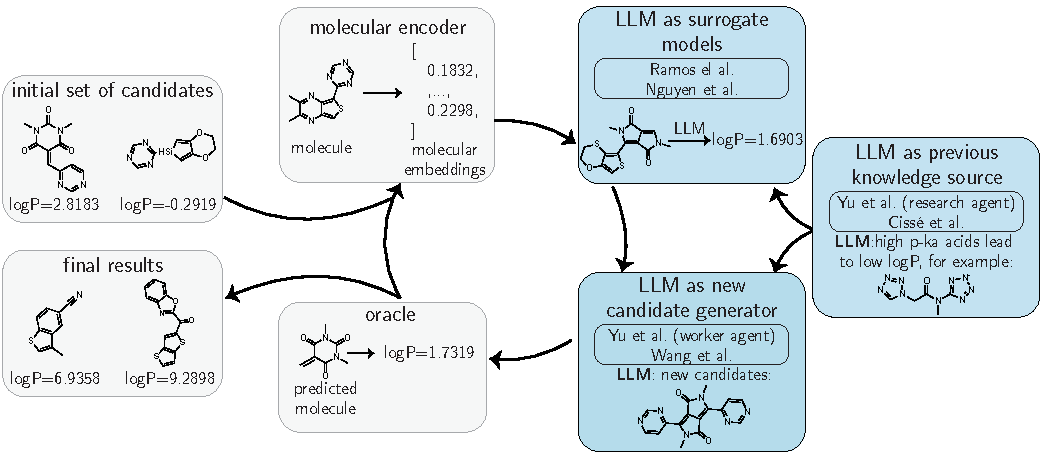
\includegraphics[width=1\textwidth]{figures/rescaled_figures/chemrev_figure22.pdf}
    \caption{\textbf{Overview of the iterative optimization loop that mirrors the structure of the optimization section}. The blue boxes contain the different roles that the \glspl{llm} play in the loop, and which are described in the main text. References in which the use of \glspl{llm} for that step are detailed inside the small boxes inside each of the components of the loop. The example shown is about obtaining molecules with high \texttt{logP}.}
    \label{fig:optimization}
\end{figure}

Discovering novel compounds and reactions in chemistry and materials science has long relied on iterative trial-and-error processes rooted in existing domain knowledge \autocite{Taylor2023brief}. While, as explained in \Cref{sec:retrosynthesis}, those methods are used to accelerate this process, optimization methods help improve conditions, binding affinity, etc.
But these approaches are slow and labor-intensive. 
Traditional data-driven methods aimed to address these limitations by combining predictive \gls{ml} models with optimization frameworks such as \gls{bo} or \glspl{ea}. 
These frameworks balance exploration of uncharted regions in chemical space with exploitation of known high-performing regions \autocite{Li2024sequential, Hse2021gryffin, Shields2021bayesian, Griffiths2020constrained, RajabiKochi2025adaptive}.

Recent advances in \glspl{llm} have unlocked potential for addressing optimization challenges in chemistry and related domains \autocite{fernando2023promptbreeder0, yang2023large, chen2024instruct}. 
A key strength of \glspl{llm} lies in their capacity to frame optimization tasks through natural language, which enhances knowledge incorporation, improves candidate comparisons, and increases interpretability. 
This aligns well with chemical problem-solving, where complex phenomena, such as reaction pathways or material behaviors, are often poorly captured by standard nomenclature; however, they can still be intuitively explained through natural language. 
Moreover, \glspl{gpm}' general capabilities provide flexibility beyond classical methods, which have to be trained from scratch if the optimization problem or any of its variables changes.
By encoding domain-specific knowledge---including reaction rules, thermodynamic principles, and structure-property relationships---into structured prompts, \glspl{llm} can synergize expertise with their ability to navigate complex chemical optimization problems.

Current \gls{llm} applications in chemistry optimization vary in scope and methodology. 
Many studies integrate \glspl{llm} into \gls{bo} frameworks, where models guide experimental design by predicting promising candidates \autocite{rankovic2023bochemian}. Others employ \glspl{ga} or hybrid strategies that combine \gls{llm}-generated hypotheses with computational screening \autocite{cisse2025language0based}.  

\subsubsection{LLMs as Surrogate Models}

A prominent \gls{llm}-driven strategy positions these models as surrogate models within optimization loops. Typically implemented as \gls{gpr}, surrogate models learn from prior data to approximate costly feature-outcome landscapes, which are often computationally and time-consuming to evaluate, thereby guiding the acquisition.
\glspl{llm} offer major advantages in this role primarily through strong low-data performance. 
Their \gls{icl} capability enables task demonstration with minimal prompt examples while leveraging chemical knowledge from pre-training to generate accurate predictions. 
This allows \glspl{gpm} to compensate for sparse experimental data effectively.

\textcite{ramos2023bayesian} demonstrated the viability of this paradigm through a simple yet effective framework that combines \gls{icl} using only one example in the prompt with a \gls{bo} workflow. 
Their \gls{bo}-\gls{icl} approach uses few-shot examples formatted as question-answer pairs, where the \gls{llm} generates candidate solutions conditioned on prior successful iterations. 
These candidates are ranked using an acquisition function, with top-$k$ selections integrated into subsequent prompts to refine predictions iteratively. 
Remarkably, this method achieved high performance in optimizing catalytic reaction conditions, even matching the top-1 accuracies observed in experimental benchmarks. This emphasizes the potential of \glspl{llm} as accessible, \gls{icl} optimizers when coupled with well-designed prompts.

To address limitations in base \glspl{llm}’ inherent chemical knowledge---particularly their grasp of specialized representations like \gls{smiles} or structure-property mappings---\textcite{yu2025collaborative} introduced a hybrid architecture augmenting pre-trained \glspl{llm} with task-specific embedding and prediction layers. 
These layers, fine-tuned on domain data, align latent representations of input-output pairs (denoted as \texttt{<x>} and \texttt{<y>} in prompts), enabling the model to map chemical structures and properties into a unified, interpretable space. Crucially, the added layers enhance chemical reasoning without sacrificing the flexibility of \gls{icl}, allowing the system to adapt to trends across iterations, similarly to what was done by \textcite{ramos2023bayesian}. 
In their evaluations of molecular optimization benchmarks, such as the \gls{pmo} \autocite{gao2022sample}, they revealed improvements over conventional methods, including \gls{bo}-\gls{gp}, \gls{rl} methods, and \gls{ga}.

\textcite{yu2025collaborative} further highlighted the framework’s extensibility to diverse black-box optimization challenges beyond chemistry. 
This represents one of the most important advantages of using \glspl{llm} as orchestrators of the optimization process. 
The flexibility of natural language in this process enables the procedure to be applied to any optimization process. 
In contrast, classical methods are constrained to the specific task for which they are designed due to the need to train the surrogate model.

\subsubsection{LLMs as Next Candidate Generators}

Recent studies demonstrate the potential of \glspl{llm} to enhance \glspl{ea} \autocite{lu2024generative} and \gls{bo} \autocite{amin2025towards} frameworks by leveraging their embedded chemical knowledge and ability to integrate prior information, thereby reducing computational effort while improving output quality.
Within \glspl{ea}, \glspl{llm} refine molecular candidates through mutations (modifying molecular substructures) or crossovers (combining parent molecules). 
In \gls{bo} frameworks, they serve as acquisition functions, utilizing surrogate model predictions---both mean and uncertainty---to select optimal molecules or reaction conditions for evaluation.

For molecule optimization, \textcite{yu2025collaborative} introduced \modelname{MultiModel}, a dual-\gls{llm} system where one model proposes candidates and the other supplies domain knowledge (see \Cref{sec:opt-llm-know-source}). 
By fine-tuning the \enquote{worker} \gls{llm} to recognize molecular scaffolds and target properties, and expanding the training pool to include a million-size pre-training dataset, they achieved hit rates exceeding $90\%$. 
Similarly, \textcite{wang2024efficient} developed \modelname{MoLLEO}, integrating an \gls{llm} into an \gls{ea} to replace random mutations with \gls{llm}-guided modifications. Here, \modelname{GPT-4} generated optimized offspring from parent molecules, significantly accelerating convergence to high fitness scores. 
Notably, while domain-specialized models (\modelname{BioT5}, \modelname{MoleculeSTM}) underperformed, the general-purpose \modelname{GPT-4} excelled---a finding that underscores the context-dependent utility of \glspl{llm}

In a related approach, \textcite{lu2024generative} showed that well-designed prompts---incorporating task-specific constraints, objectives, and few-shot examples---enable general \glspl{llm} (\modelname{Claude\--3.5-Sonnet}, \modelname{o1-preview}) to generate high-quality candidates without fine-tuning, outperforming both random selection and vanilla \glspl{ga} in functional \gls{tmc} design.

\subsubsection{LLMs as Prior Knowledge Sources} \label{sec:opt-llm-know-source}

A key advantage of integrating \glspl{llm} into optimization frameworks is their ability to encode and deploy prior knowledge within the optimization loop. 
As illustrated in \Cref{fig:optimization}, this knowledge can be directed into either the surrogate model or candidate generation module, significantly reducing the number of optimization steps required through high-quality guidance.

For example, \textcite{yu2025collaborative} deployed a \enquote{research} agent that leverages \modelname{Google} search and \modelname{RDKit} to verify and rank molecules generated by \enquote{worker} agents against target features and properties. 
Their results demonstrate substantial improvements when this filtering mechanism is applied.

Similarly, \textcite{cisse2025language0based} introduced \modelname{BORA}, which contextualizes conventional black-box \gls{bo} using an \gls{llm}. \modelname{BORA} maintains standard \gls{bo} as the core driver but strategically activates the \gls{llm} when progress stalls. 
This leverages the model’s \gls{icl} capabilities to hypothesize promising search regions and propose new samples, regulated by a lightweight heuristic policy that manages costs and incorporates domain knowledge (or user input). 
Evaluations on synthetic benchmarks such as the catalyst optimization task for hydrogen generation show that \modelname{BORA} accelerates exploration, improves convergence, and outperforms existing \gls{llm}-\gls{bo} hybrids.

To enhance the task-specific knowledge of the \gls{llm} generating feedback, \textcite{zhang2025large} fine-tuned a \modelname{Llama-2-7B} model using a multitask \gls{qa} dataset. This dataset was created with instructions from \modelname{GPT-4}. 
The resulting model served as a human assistant or operated within an active learning loop, thereby accelerating the exploration of new reaction spaces (see \Cref{sec:retrosynthesis}). 
However, as the authors note, even this task-specialized \glspl{llm} produces suboptimal suggestions for optimization tasks. 
They remain prone to hallucination and cannot assist with unreported reactions, but still, they improve for most of the applications, using pure classical methods.

\subsubsection{How to Face Optimization Problems?}

Published works explore different ways of using \glspl{llm} for optimization problems in chemistry, from simple approaches, such as just prompting the model with some initial random set of experimental candidates and iterating \autocite{ramos2023bayesian}, to fine-tuning models in \gls{bo} fashion \autocite{rankovic2025gollum0}. 
The most efficient initial point is by relying entirely on a \gls{icl} approach, which allows one to obtain a first signal rapidly. 
Such initial results will enable to determine whether a more complex, computationally intensive approach is necessary or whether prompt engineering is reliable enough for the application. 
Fine-tuning can be used as a way to enhance the chemical knowledge of the \glspl{llm} and can lead to improvements in optimization tasks where the model requires such knowledge to choose or generate better candidates. 
Fine-tuning might not be a game-changer for other approaches that rely more on sampling methods \autocite{wang2025llm0augmented}.

While some initial works showed that \glspl{llm} trained specifically on chemistry perform better for optimization tasks \autocite{kristiadi2024sober}, other works showed that a \gls{gpm} such as \modelname{GPT-4} combined with an \gls{ea} outperformed all other models \autocite{wang2024efficient}.
Is it better to incorporate a general model or a chemistry \gls{lm} into the optimization frameworks?
We hypothesize that for models of the same size (in number of parameters) and similar training size---attending to \glspl{pflop}---a chemical \gls{lm} (a specialized model) will consistently outperform general models. 
If the models differ significantly in size, the larger model will typically perform better.

